%%Seitenumbruch
%%\enlargethispage{2\baselineskip} 

% Konfigurationsdatei f\"ur die Pfaddefinitionen einlesen
%  se-wa-pfade.tex
%
%
%  J\"org Baumgart
%  2012-12-20
%  
%  Pfaddefinitionen (Ordnerdefinitionen) f\"ur das Einlesen von
%  -- .sty-Dateien und
%  -- Textbaustenen f\"ur die Hinweise zur Verwendung von LaTeX
%  -- jpg-Bildern
%
\newcommand{\seWaPathSty}{se-wa-styles}
\newcommand{\seWaPathText}{se-wa-textbausteine-vorlagen}
\newcommand{\seWaPathJpg}{se-wa-jpg}

%
%
% Festlegung der Sprache: 
\newcommand{\seWaSprache}{deutsch}
%\newcommand{\seWaSprache}{englisch}

%
% Einlesen der .sty-Dateien
%
%  se-wa-input-styles-v098.tex
%
%  Joerg Baumgart 01.08.2011
%
%  Zusammenfassung und Konfiguration wichtiger Styles f\"ur die 
%  Erzeugung von Seminar-, Projekt- und Bachelorarbeiten
%
%  2012-03-12: auf Version 0.94 umgestellt
%
%
% 2012-12-13: auf Version 0.95 umgestellt
%                     Sprachoptionen englisch/deutsch zusammengef\"uhrt
%                     bchart.sty hinzugenommen
%                 
%
% 2013-01-27: auf Version 0.96 umgestellt
%                     algorithm2e-Paket integriert
%
%
% 2013-07-08: auf Version 0.97 umgstellt 
%                     utf8, Fehlerkorrekturen bei pa1
%
% 2014-02-02: auf Version 0.971 umgestellt
%                     Workaround für Fehler im KOMAScript 3.2
%                     KOMAoption listof un documentclass übernommen
%
%
%
%
% 2014-07-22: etex-Paket hinzugenommen
%
%
% 2016-04-01: Sperrvermerk und Ehrenwörtliche Erklärung aus der PO 2015
%
%
%
% 2016-12-18: auf Version 0.98 umgestellt
%                     bchart.sty und algorithm2e haben veraltete Kommandos verwendet (\sf und \bf), 
%                     die unter MacTeX 2016 nicht mehr unterstützt werden 
%

\documentclass[12pt,BCOR=10mm,headinclude=on,footinclude=off,bibliography=totoc,listof=ignorechapter]{scrreprt}
\usepackage{etex}
\usepackage[T1]{fontenc}
\usepackage[utf8]{inputenc}
\usepackage{ifthen}
% 2012-12-13
\ifthenelse{\equal{\seWaSprache}{deutsch}}{% Deutsche Einstellungen
\usepackage[ngerman]{babel}% 
}{% Englische Einstellungen
\usepackage[english]{babel}% 
}

\usepackage{lmodern}

\usepackage{tikz} % Graphikpaket, das zu pdfLaTeX kompatibel ist
\usepackage{xkeyval} % Definition von Kommandos mit mehreren optionalen Argumenten
\usepackage{listings} % Formatierung von Programmlistings
\usepackage{graphicx} % Einbinden von Graphiken
\usepackage{color}
\usepackage{\seWaPathSty/slashbox} % Diagonalen in Tabellenfeldern
\usepackage{framed} % Erzeugung schwarzer Linien am linken Rand zur Hervorhebung von Textteilen
\usepackage{caption} % Korrektes Setzen einer mehrzeiligen float-Unterschrift bei neu definierten float-Umgebungen
\usepackage{floatrow}
% 2012-12-13
\usepackage{\seWaPathSty/bchart} % Kommandos zur Erzeugung von Balkendiagrammen
% 2013-01-27 
\usepackage[boxed,ngerman]{\seWaPathSty/algorithm2e}
%\usepackage[tworuled,vlined,ngerman]{\seWaPathSty/algorithm2e}


% Es wird jeweils die sty-Datei importiert und entsprechende Konfigurationseinstellungen werden vorgenommen

\usepackage{\seWaPathSty/se-jb-scrpage2} % Formatierung der Kopf- und Fu{\ss}zeilen
\usepackage{\seWaPathSty/se-jb-footmisc}    % Fussnoten besser formatieren

\usepackage{\seWaPathSty/se-jb-glossaries-v097} % Abk\"urzungsverzeichnis, Symbolverzeichnis, Glossar
   
\usepackage{\seWaPathSty/se-jb-floatrow}    % Definition und Konfiguration von float-Umgebungen (figure, table, die neue programm-Umgebung)
% Achtung: se-jb-varioref muss nach se-jb-floatrow importiert werden; 
% andernfalls ist der counter programm f\"ur die labelformat-Anweisung noch nicht definiert   
\usepackage{\seWaPathSty/se-jb-varioref-v097}   % Definition von Querverweisen
\usepackage{\seWaPathSty/se-jb-chngcntr}   % Kapitelweise oder globale Nummerierung von Abbildungen etc.
   
\usepackage{\seWaPathSty/se-jb-listen} % Definition neuer, besser formatierter Listen
% 2014-02-02
%\usepackage{\seWaPathSty/se-jb-kommandos-v097} % neue Kommandos f\"ur Seminar-, Projekt- und Bachelorarbeiten
%\usepackage{\seWaPathSty/se-jb-kommandos-v0971} % neue Kommandos f\"ur Seminar-, Projekt- und Bachelorarbeiten
% 2016-04-01
\usepackage{\seWaPathSty/se-jb-kommandos-v0972} % neue Kommandos f\"ur Seminar-, Projekt- und Bachelorarbeiten
% 2012-12-13
\ifthenelse{\equal{\seWaSprache}{englisch}}{\usepackage{\seWaPathSty/se-jb-kommandos-englisch-v0972}}{}

% 2016-12-18
\renewcommand{\sf}{\sffamily}
\renewcommand{\bf}{\bfseries}



\lstdefinelanguage{JavaScript}{
keywords={typeof, new, true, false, catch, function, return, null, catch, switch, var, if, in, while, do, else, case, break, \$.},
keywordstyle=\color{blue}\bfseries,
ndkeywords={class, export, boolean, throw, implements, import, this},
ndkeywordstyle=\color{darkgray}\bfseries,
identifierstyle=\color{black},
sensitive=false,
comment=[l]{//},
morecomment=[s]{/*}{*/},
commentstyle=\color{purple}\ttfamily,
stringstyle=\color{blue}\ttfamily,
morestring=[b]',
morestring=[b]"
}

\lstset{
language=JavaScript,
backgroundcolor=\color{white},
extendedchars=true,
basicstyle=\footnotesize\ttfamily,
showstringspaces=false,
showspaces=false,
numbers=left,
numberstyle=\footnotesize,
numbersep=9pt,
tabsize=2,
breaklines=true,
showtabs=false,
captionpos=b
}

\usepackage{xcolor}

\colorlet{punct}{red!60!black}
\definecolor{delim}{RGB}{20,105,176}
\colorlet{numb}{magenta!60!black}

\lstdefinelanguage{json}{
    basicstyle=\normalfont\ttfamily,
    numbers=left,
    numberstyle=\scriptsize,
    stepnumber=1,
    numbersep=8pt,
    showstringspaces=false,
    breaklines=true,
    frame=lines,
    backgroundcolor=\color{white},
    literate=
     *{0}{{{\color{numb}0}}}{1}
      {1}{{{\color{numb}1}}}{1}
      {2}{{{\color{numb}2}}}{1}
      {3}{{{\color{numb}3}}}{1}
      {4}{{{\color{numb}4}}}{1}
      {5}{{{\color{numb}5}}}{1}
      {6}{{{\color{numb}6}}}{1}
      {7}{{{\color{numb}7}}}{1}
      {8}{{{\color{numb}8}}}{1}
      {9}{{{\color{numb}9}}}{1}
      {:}{{{\color{punct}{:}}}}{1}
      {,}{{{\color{punct}{,}}}}{1}
      {\{}{{{\color{delim}{\{}}}}{1}
      {\}}{{{\color{delim}{\}}}}}{1}
      {[}{{{\color{delim}{[}}}}{1}
      {]}{{{\color{delim}{]}}}}{1},
}


%
% Individuelle Konfiguration des Dokumentes
%
%  Individuelle Konfiguration einer Projektarbeit/Bachelorarbeit
%
%
%
%

% 2012-10-27
%
% \"Anderung des Schrifttyps f\"ur das gesamte Dokument
%
% Das gesamte Dokument wird in einer serifenlosen Schrift gesetzt
%\renewcommand{\familydefault}{\sfdefault}
%
% Das gesamte Dokument wird in einer Serifenschrift gesetzt
% Achtung: serifenlose Schriften sind jetzt grunds\"atzlich nicht mehr nutzbar!
%
%\renewcommand{\sffamily}{\normalfont}

% 2012-12-05
%
% Verwendung des url-Pakets
% Durch den optionalen Paremeter hyphens wird eine Trennung 
% von URLs auch nach Bindestrichen erlaubt
\usepackage[hyphens]{url}


% 2012-10-27
%
%
% Literaturverzeichnis
% 
% Literaturverzeichnis gem\"ass den Vorgaben von Theisen aufbauen
\usepackage{\seWaPathSty/se-jb-jurabib-theisen} 
% Verwendung der Harvard-Zitierweise
%\usepackage{\seWaPathSty/se-jb-jurabib-harvard} 

% Weitere Optionseinstellungen f\"ur das Koma-Script
%
% Zwischen Abs\"atzen einen Abstand von 0.5 \baselineskip erzeugen
\KOMAoption{parskip}{full}
%
% Vergleiche Duden "Gliederung von Nummern, S.111" 
% DIN 5008 anschauen, wenn sie neu ver\"offentlicht wurde
\KOMAoption{numbers}{noendperiod}
%
%



%  Voreinstellungen f\"ur floats
%  Durch die verwendeten Parameter wird die Wahrscheinlichkeit deutlich kleiner, 
%  dass Gleitobjekte (z. B. Abbildungen) ans Ende des Dokumentes verschoben 
%  werden; 
%  Achtung: clearpage erzwingt die Ausgabe von Gleitobjekten
%
\renewcommand{\topfraction}{1}  % Gleitobjekte d\"urfen eine Seite zu 100% belegen 
\renewcommand{\bottomfraction}{1} % Entsprechender Wert f\"ur den unteren Teil der Seite
\renewcommand{\textfraction}{0} % Eine Seite darf auch ohne Fliesstext existieren
%%%\renewcommand{\floatpagefraction}{1} % Bedeutung unklar, daher keine Ver\"anderung des Vorgabewertes 
                                                                        % von 0.5; eventuell bringt ein \"Anderung auf 1 etwas, wenn 
                                                                         % Probleme mit floats auftreten
                                                                         
                                                                         
                                                                         
% Konfiguration von Programm-Listings
% 
% Achtung: hier gibt es nahezu beliebig viele weitere Konfigurationm\"oglichkeiten; vgl. Paketdokumentation
%
\lstset{language=Java,basicstyle=\ttfamily,keywordstyle=\color{blue},captionpos=b,aboveskip=0mm,belowskip=0mm,
          xleftmargin=0em}               
          
%
% Grundkonfiguration der Abs\"ande zwischen den Items der maximal f\"unf Verschachtelungsebenen der 
% neuen Listenumgebungen
%                                                                             
% Initialisierung der Abst\"ande zwischen den items f\"ur seList; Grundeinheit: 0.5\baselineskip; siehe se-jb-listen
\seSetlistbaselineskip{1}{0.75}{0.75}{0.75}{0.75}
% Initialisierung der Abst\"ande zwischen den items f\"ur seToplist; Grundeinheit: 0.5\baselineskip; siehe se-jb-listen
\seSettoplistbaselineskip{1}{0.75}{0.75}{0.75}{0.75}     


% Einlesen der sprachabh\"angigen Konfigurationsdatei
%
%
\ifthenelse{\equal{\seWaSprache}{deutsch}}{% deutsch
% wa-konfiguration-deutsch
%
% 2012-12-13
% 
% Diese Datei wird f\"ur die Sprachoption deutsch verwendet, d. h.  
% \newcommand{\seWaSprache}{deutsch}
%
%
% In dieser Datei k\"onnen Neudefinitionen vorgenommen werden f\"ur:
% -- Verzeichnisse
% -- Unter-/\"Uberschriften von Abbildungen, Tabellen und Listings
% -- Querverweise innerhalb des Textes

% 2013-01-26: Konfiguration des Algorithmenverzeichnis
%
%
%

% 2013-07-08: Querverweis auf Anhang hinzugenommen
%
%
%


%
%  Konfiguration der verschiedenen Verzeichnisse
%
%  abstandEintrag: Wert wird mit \baselineskip multipliziert
%

%
%  Abbildungsverzeichnis
%
\seKonfigurationAbb[
%verzeichnisname=Abbildungsverzeichnis,
labeltextLinks=, % kein Text links;
%labeltextRechts=:,
labelbreite=1cm,
%labeleinzug=1cm,
%abstandEintrag=1,
%newpage=ja,
%pnumwidth=20mm,
%dotsep=1000,
%tocrmarg=4.5cm,
%abstandVerzeichnis=-1mm
]

%
% LIstingverzeichnis
%
\seKonfigurationPrg[
%verzeichnisname=Listing-Verzeichnis,
labeltextLinks=,
%labeltextRechts=:,
labelbreite=1cm,
%labeleinzug=2cm,
%abstandEintrag=1,
%newpage=ja,
%pnumwidth=20mm,
%dotsep=1000,
%tocrmarg=4.5cm,
%abstandVerzeichnis=-10mm
]

% 2013-01-26
%
% Algorithmenverzeichnis
%
\seKonfigurationAlg[
%verzeichnisname=Algorithmen-Verzeichnis,
labeltextLinks=,
%labeltextRechts=:,
labelbreite=1cm,
%labeleinzug=2cm,
%abstandEintrag=1,
%newpage=ja,
%pnumwidth=20mm,
%dotsep=1000,
%tocrmarg=4.5cm,
%abstandVerzeichnis=-10mm
]




%
% Tabellenverzeichnis
%
\seKonfigurationTab[
%verzeichnisname=Liste der Tabellen,
labeltextLinks=,
%labeltextRechts=:,
labelbreite=1cm,
%labeleinzug=0.5cm,
%abstandEintrag=1,
%newpage=ja,
%pnumwidth=20mm,
%dotsep=1000,
%tocrmarg=4.5cm,
%abstandVerzeichnis=-10mm
]

%
% Abk\"urzungsverzeichnis
%
\seKonfigurationAbk[
%verzeichnisname=Liste der Abk\"urzungen,
%labelbreite=3cm,
%labeleinzug=0.5cm,
%abstandEintrag=1,
%newpage=ja,
%abstandVerzeichnis=-10mm
]

%
% Symbolverzeichnis
% 
\seKonfigurationSym[
%verzeichnisname=Liste der Symbole,
%labelbreite=4cm,
%labeleinzug=3.5cm,
%abstandEintrag=1,
%newpage=ja,
%abstandVerzeichnis=-10mm
]

%
% Glossar
%
\seKonfigurationGlo[
%verzeichnisname=Glossar,
%abstandEintrag=0,
]



% (eventuelle) Neudefinition f\"ur die Unter-/\"Uberschriften von Abbildungen, Tabellen und Listings
%
%
%\renewcommand{\seCaptionNameAbbildung}{Abb.}
%\renewcommand{\seCaptionNameTabelle}{Tab.}
%\renewcommand{\seCaptionNameProgramm}{Prg.}


% % (eventuelle) Neudefinition f\"ur Querverweise innerhalb des Textes
%
%
%
%\renewcommand{\seQuerverweisSeite}{Seite}
%\renewcommand{\seQuerverweisAbbildung}{Abb.}
%\renewcommand{\seQuerverweisTabelle}{Tab.}
%\renewcommand{\seQuerverweisProgramm}{Prg.}
%\renewcommand{\seQuerverweisGleichung}{Gl.}
%\renewcommand{\seQuerverweisAlgorithmus}{Alg.}
%
\renewcommand{\seQuerverweisChapter}{Kapitel}
% 2013-07-08
\renewcommand{\seQuerverweisAppendix}{Anhang}
\renewcommand{\seQuerverweisSection}{Kapitel}
\renewcommand{\seQuerverweisSubsection}{Kapitel}
\renewcommand{\seQuerverweisSubsubsection}{Kapitel}
\renewcommand{\seQuerverweisParagraph}{Kapitel}


%
% Kommandos f\"ur die Konfiguration von URL-Eintr\"agen im Literaturverzeichnis
%
\renewcommand*{\biburlprefix}{\jblangle{}URL: }
\renewcommand*{\biburlsuffix}{\jbrangle{}}
\renewcommand*{\bibbudcsep}{ -- }
\AddTo\bibsgerman{\renewcommand*{\urldatecomment}{Zugriff am }}


%
}{% englisch
% wa-konfiguration-englisch
%
% 2012-12-13
% 
% Diese Datei wird f\"ur die Sprachoption englisch verwendet, d. h.  
% \newcommand{\seWaSprache}{englisch}
%
%
% In dieser Datei k\"onnen Neudefinitionen vorgenommen werden f\"ur:
% -- Verzeichnisse
% -- Unter-/\"Uberschriften von Abbildungen, Tabellen und Listings
% -- Querverweise innerhalb des Textes

% 2013-07-08: Querverweis auf Anhang hinzugenommen
%
%
%


%
%  Konfiguration der verschiedenen Verzeichnisse
%
%  abstandEintrag: Wert wird mit \baselineskip multipliziert
%

%
%  Abbildungsverzeichnis
%
\seKonfigurationAbb[
verzeichnisname=List of Figures,
labeltextLinks=, % kein Text links;
%labeltextRechts=:,
labelbreite=1cm,
%labeleinzug=1cm,
%abstandEintrag=1,
%newpage=ja,
%pnumwidth=20mm,
%dotsep=1000,
%tocrmarg=4.5cm,
%abstandVerzeichnis=-1mm
]

%
% LIstingverzeichnis
%
\seKonfigurationPrg[
verzeichnisname=List of Program Listings,
labeltextLinks=,
%labeltextRechts=:,
labelbreite=1cm,
%labeleinzug=2cm,
%abstandEintrag=1,
%newpage=ja,
%%pnumwidth=20mm,
%dotsep=1000,
%tocrmarg=4.5cm,
%abstandVerzeichnis=-10mm
]


% 2013-01-26
%
% Algorithmenverzeichnis
%
\seKonfigurationAlg[
verzeichnisname=List of Algorithms,
labeltextLinks=,
%labeltextRechts=:,
labelbreite=1cm,
%labeleinzug=2cm,
%abstandEintrag=1,
%newpage=ja,
%pnumwidth=20mm,
%dotsep=1000,
%tocrmarg=4.5cm,
%abstandVerzeichnis=-10mm
]


%
% Tabellenverzeichnis
%
\seKonfigurationTab[
verzeichnisname=List of Tables,
labeltextLinks=,
%labeltextRechts=:,
labelbreite=1cm,
%labeleinzug=0.5cm,
%abstandEintrag=1,
%newpage=ja,
%pnumwidth=20mm,
%dotsep=1000,
%tocrmarg=4.5cm,
%abstandVerzeichnis=-10mm
]

%
% Abk\"urzungsverzeichnis
%
\seKonfigurationAbk[
verzeichnisname=List of Abbreviations,
%labelbreite=3cm,
%labeleinzug=0.5cm,
%abstandEintrag=1,
%newpage=ja,
%abstandVerzeichnis=-10mm
]

%
% Symbolverzeichnis
% 
\seKonfigurationSym[
verzeichnisname=List of Symbols,
%labelbreite=4cm,
%labeleinzug=3.5cm,
%abstandEintrag=1,
%newpage=ja,
%abstandVerzeichnis=-10mm
]

%
% Glossar
%
\seKonfigurationGlo[
verzeichnisname=Glossary,
%abstandEintrag=0,
]



% (eventuelle) Neudefinition f\"ur die Unter-/\"Uberschriften von Abbildungen, Tabellen und Listings
%
%
\renewcommand{\seCaptionNameAbbildung}{Figure}
\renewcommand{\seCaptionNameTabelle}{Table}
\renewcommand{\seCaptionNameProgramm}{Listing}
\renewcommand{\seCaptionNameAlgorithmus}{Algorithm}


% % (eventuelle) Neudefinition f\"ur Querverweise innerhalb des Textes
%
%
%
\renewcommand{\seQuerverweisSeite}{page}
\renewcommand{\seQuerverweisAbbildung}{figure}
\renewcommand{\seQuerverweisTabelle}{table}
\renewcommand{\seQuerverweisProgramm}{listing}
\renewcommand{\seQuerverweisGleichung}{equation}
\renewcommand{\seQuerverweisAlgorithmus}{algorithm}
%
\renewcommand{\seQuerverweisChapter}{chapter}
\renewcommand{\seQuerverweisAppendix}{appendix}
\renewcommand{\seQuerverweisSection}{chapter}
\renewcommand{\seQuerverweisSubsection}{chapter}
\renewcommand{\seQuerverweisSubsubsection}{chapter}
\renewcommand{\seQuerverweisParagraph}{chapter}


%
% Kommandos f\"ur die Konfiguration von URL-Eintr\"agen im Literaturverzeichnis
%
\renewcommand*{\biburlprefix}{\jblangle{}URL: }
\renewcommand*{\biburlsuffix}{\jbrangle{}}
\renewcommand*{\bibbudcsep}{ -- }
\AddTo\bibsenglish{\renewcommand*{\urldatecomment}{visited on }}


}

% Kommandos, die direkt nach \begin{document} ausgef\"uhrt werden m\"ussen
%
%
%
\AtBeginDocument{%
\renewcommand{\listfigurename}{\seAbbildungenVerzeichnisname}
\renewcommand{\listtablename}{\seTabellenVerzeichnisname}
\renewcommand{\figurename}{\seCaptionNameAbbildung}
\renewcommand{\tablename}{\seCaptionNameTabelle}
\labelformat{lstlisting}{\seQuerverweisProgramm{} #1}
\renewcommand{\thelstlisting}{\theprogramm}
\pagenumbering{roman}
}
                                                              
                                                                         

%
% Definition von Abk\"urzungen, Symbolen und eventuell Glossareintr\"agen
%
% 2012-03-22 Verwendung des optionalen Parameters f\"ur die Pluralform einer Abk\"urzung
%
% 2012-02-06 Umstellung auf die neuen Kommandos
%
%
%
%  J\"org Baumgart
%  Definition einiger Abk\"urzungen
%  


% Definition von Abk\"urzungen
%
% 1. Parameter: Schluessel (key) der Abkuerzung
% 2. Parameter: Abkuerzung
% 3. Parameter: Vollform
% 4. Parameter: Vollform im Plural (optional; falls nicht definiert, wird der Wert des dritten Parameters verwendet)
%

\seNewAcronymEntry{dhbw}{DHBW}{Duale Hochschule Baden-W\"urttemberg}{}{}

\seNewAcronymEntry{usb}{USB}{Universal Serial Bus}{}

\seNewAcronymEntry{ctan}{CTAN}{Comprehensive \TeX{} Archive Network}{}

\seNewAcronymEntry{sap}{SAP}{eigenständiger Markenname - früher: \textit{Systeme, Anwendungen und Produkte in der Datenverarbeitung}}{}

\seNewAcronymEntry{mvc}{MVC}{Model-View-Controller}{}

\seNewAcronymEntry{vba}{VBA}{Visual Basic for Applications}{}

\seNewAcronymEntry{erp}{ERP}{Enterprise Resource Planing}{}

\seNewAcronymEntry{ui}{UI}{User Interface}{}

\seNewAcronymEntry{html}{HTML}{Hypertext Markup Language}{}

\seNewAcronymEntry{svg}{SVG}{Scalable Vector Graphics}{}

\seNewAcronymEntry{dom}{DOM}{Document Object Model}{}

\seNewAcronymEntry{xml}{XML}{Extensible Markip Language}{}

\seNewAcronymEntry{css}{CSS}{Cascading Style Sheets}{}

\seNewAcronymEntry{jpg}{JPEG}{Joint Photographic Expters Group}{}

\seNewAcronymEntry{png}{PNG}{Portable Network Graphics}{}

\seNewAcronymEntry{w3c}{W3C}{World Wide Web Consortium}{}

\seNewAcronymEntry{d3}{D3}{Data Driven Document}{}

\seNewAcronymEntry{kpi}{KPI}{Key Perfomance Indicator}{}

\seNewAcronymEntry{oss}{OSS}{Open Source Software}{}

\seNewAcronymEntry{osi}{OSI}{Open Source Initiative}{}

\seNewAcronymEntry{c4a}{C4A}{Cloud for Analytics}{}

\seNewAcronymEntry{mit}{MIT}{Massachusetts Institute of Technology}{}

\seNewAcronymEntry{wtfpl}{WTFPL}{WHAT THE FUCK PUBLIC LICENSE}{}

\seNewAcronymEntry{json}{JSON}{JavaScript Object Notation}{}

%\seNewAcronymEntry{kdd}{KDD}{Knowledge Discovery in Data}{}

%\seNewAcronymEntry{dm}{DM}{Data Mining}{}

%\seNewAcronymEntry{crisp-dm}{CRISP-DM}{Cross Industry Standard Process for Data Mining}{}

%\seNewAcronymEntry{iot}{IoT}{Internet of Things}{}


%\seNewAcronymEntry{olap}{OLAP}{Online Analytical Processing}{}

%\seNewAcronymEntry{sql}{SQL}{Structured Query Language}{}

%\seNewAcronymEntry{knn}{KNN}{K-Nearest Neighbours}{}
\seNewAcronymEntry{matlab}{MATLAB}{MATrix LABoratory}{}

\seNewAcronymEntry{rss}{RSS}{Residual Sum of Squares}{}


\seNewAcronymEntry{tss}{TSS}{Total Sum of Squares}{}

\seNewAcronymEntry{cft}{CFT}{Curve Fitting Tool}{}



\seNewAcronymGlossaryEntry{ml}{ML}{Machine Learning}%
{}%
{Definition folgt}

\seNewAcronymGlossaryEntry{olap}{OLAP}{Online Analytical Processing}%
{}%
{Definition folgt}

\seNewAcronymGlossaryEntry{sql}{SQL}{Structured Query Language}%
{}%
{Definition folgt}

\seNewAcronymGlossaryEntry{knn}{KNN}{K-Nearest Neighbours}%
{}%
{Definition folgt}

\seNewAcronymGlossaryEntry{dm}{DM}{Data Mining}%
{}%
{Definition folgt}

\seNewAcronymGlossaryEntry{iot}{IoT}{Internet of Things}%
{}%
{Definition folgt}

\seNewAcronymGlossaryEntry{crisp-dm}{CRISP-DM}{Cross Industry Standard Process for Data Mining}%
{}%
{Definition folgt}

\seNewAcronymGlossaryEntry{kdd}{KDD}{Knowledge Discovery in Data}%
{}%
{Definition folgt}

\seNewAcronymGlossaryEntry{svm}{SVM}{Super Vector Machine}%
{}%
{Definition folgt}

\seNewAcronymGlossaryEntry{nn}{NN}{Neuronale Netze}%
{}%
{Definition folgt}

\seNewAcronymGlossaryEntry{mdkq}{MDKQ}{Methode der kleinsten Quadrate}%
{}%
{Definition folgt}

\seNewGlossaryEntry{bigdata}{Big Data}{}{Definition folgt}

\seNewGlossaryEntry{clustering}{Clustering}{}{Definition folgt}

\seNewGlossaryEntry{regression}{Regression}{}{Definition folgt}

\seNewGlossaryEntry{outlier}{Outlier Detection}{}{Definition folgt}

\seNewGlossaryEntry{ki}{Künstliche Intelligenz}{Künstlichen Intelligenz}{Definition folgt}



% 2012-03-24
% \"Uber den optionalen Parameter in eckigen Klammern wird die Pluralform f\"ur das erste 
% Auftreten der Abk\"urzung definiert

\seNewAcronymEntry[URLs]{url}{URL}{Uniform Resource Locator}%
{Uniform Resource Locators}


% Definition von Symbolen
%
% 1. Parameter: Schluessel (key) des Symbols
% 2. Parameter: Symbol
% 3. Parameter: Text, der die Sortierreihenfolge festlegt (optional; falls nicht definiert, wird der Wert des zweiten 
%                        Parameters verwendet)
% 4. Parameter: Beschreibung des Symbols
%

\seNewSymbolEntry{ND}{ND}{a}{Nutzungsdauer einer Maschine}

\seNewSymbolEntry{pi}{$\pi$}{b}{Die Kreiszahl}




% Definition von Glossareintraegen
%
% 1. Parameter: Schluessel (key) des Glossareintrags
% 2. Parameter: Begriff, der im Glossar definiert wird
% 3. Parameter: Pluralform des Begriffes (optional; falls nicht definiert, wird der Wert des zweiten Parameters verwendet)
%                        Achtung: Pluralform gilt nur fuer das erste Auftreten des Begriffes im Text
% 4. Parameter: Beschreibung des Glossareintrags
%
%
%

\seNewGlossaryEntry{glos:AD}{Active Directory}{Active Directories}
{Active Directory ist in einem Windows 2000/Windows
Server 2003-Netzwerk der Verzeichnisdienst, der die zentrale
Organisation und Verwaltung aller Netzwerkressourcen erlaubt. Es
erm\"oglicht den Benutzern \"uber eine einzige zentrale Anmeldung den
Zugriff auf alle Ressourcen und den Administratoren die zentral
organisierte Verwaltung, transparent von der Netzwerktopologie und
den eingesetzten Netzwerkprotokollen. Das daf\"ur ben\"otigte
Betriebssystem ist entweder Windows 2000 Server oder
Windows Server 2003, welches auf dem zentralen
Dom\"anencontroller installiert wird. Dieser h\"alt alle Daten des
Active Directory vor, wie z.\,B. Benutzernamen und
Kennw\"orter.\protect\footnote{Bedauerlicherweise wei{\ss} der Autor dieses Dokumentes nicht mehr, woher diese Information stammt -- das 
geht in einer richtigen wissenschaftlichen Arbeit nat\"urlich \"uberhaupt nicht!!!}}
%\protect\seFootcite{Vgl.}{S. 200}{Dud09}}


\seNewGlossaryEntry{glos:bs}{Betriebssystem}{Betriebssysteme}{Die Begriffsdefinition sollten Sie eigentlich kennen!}



% Definition von Glossareintraegen, die gleichzeitig im Abk�rzungsverzeichnis auftreten
%
% 1. Parameter: Schluessel (key) des Glossareintrags
% 2. Parameter: Abk\"urzung
% 3. Parameter: Vollform
% 4. Parameter: Vollform im Plural (optional; falls nicht definiert, wird der Wert des dritten Parameters verwendet)
% 5. Parameter: Beschreibung des Glossareintrags

\seNewAcronymGlossaryEntry{glos:ma}{MA}{Mobile Applikation}{Mobile Applikationen}
{Eine Applikation, die auf einem mobilen Endger\"at ausgef\"uhrt wird.}

% 2012-03-24
% \"Uber den optionalen Parameter in eckigen Klammern wird die Pluralform f\"ur die Abk\"urzung definiert

\seNewAcronymGlossaryEntry[TAen]{glos:ta}{TA}{Transaktion}%
{Transaktionen}%
{Was eine Transaktion ist, sollten Sie ebenfalls bereits wissen!}





% Alternative Definition von Abk\"urzungen; diese sollten nicht verwendet werden!!!
%
%\newacronym{dhbw}{DHBW}{Duale Hochschule Baden-W\"urttemberg}
%\newacronym{usb}{USB}{Universal Serial Bus}


% Alternative Definition von Symbolen
%
% Achtung: ohne sort wird nach Name sortiert
%\newglossaryentry{pi}{
%name=$\pi$,
%description={Die Kreiszahl},
%type=symbolslist,
%sort=b
%}
%
%\newglossaryentry{ND}{
%name=$\mbox{\textsl{ND}}$,
%description={Nutzungsdauer einer Maschine},
%type=symbolslist,%
%sort=a
%}



% Alternative Definition von Glossareintr\"agen
%
%\newglossaryentry{glos:AD}{
%first=Active Directory\textsuperscript{GL},
%name=Active Directory,
%description={Active Directory ist in einem Windows 2000/Windows
%Server 2003-Netzwerk der Verzeichnisdienst, der die zentrale
%Organisation und Verwaltung aller Netzwerkressourcen erlaubt. Es
%erm\"oglicht den Benutzern \"uber eine einzige zentrale Anmeldung den
%Zugriff auf alle Ressourcen und den Administratoren die zentral
%organisierte Verwaltung, transparent von der Netzwerktopologie und
%den eingesetzten Netzwerkprotokollen. Das daf\"ur ben\"otigte
%Betriebssystem ist entweder Windows 2000 Server oder
%Windows Server 2003, welches auf dem zentralen
%Dom\"anencontroller installiert wird. Dieser h\"alt alle Daten des
%Active Directory vor, wie z.\,B. Benutzernamen und
%Kennw\"orter.\protect\seFootcite{Vgl.}{S. 200}{Dud09}}
%}














 

%\seIstErsteProjektarbeit{}
%\seIstZweiteProjektarbeit{}
\seIstBachelorarbeit{}

\newcommand{\version}{0.98}

% 
% Diese Redefinition ist nur f\"ur den Anhang B der  
% Vorlage (Hinweise zur Installation und \"Ubersetzung)
% notwendig; f\"ur Ihre Bachelorarbeit spielt sie keine Rolle
%
\renewcommand{\seVorlage}{\jobname}
\usepackage{color}
\usepackage{pgfplots}
\usepackage{amssymb} 
\usetikzlibrary{decorations.pathreplacing}
\usepackage{rotating}
\usepackage{pifont}
\usepackage{pdflscape}
\usepackage{pdfpages} 
\usepackage{tabularx}
\usepackage{tabularx}
\usepackage{array}
\newcolumntype{P}[1]{>{\centering\arraybackslash}p{#1}}


\begin{document}

% Erzeugung des Titelblatts
%
%
%
\seTitelblattWissenschaftlicheArbeit[
%hilfslinien=ja,
%dhbwlogoSkalierung=0.5,
%dhbwlogoDeltaX=2.4,
%dhbwlogoDeltaY=-10,
firmenlogo=firmenlogo,
firmenlogoSkalierung=0.175,
firmenlogoDeltaX=0,
firmenlogoDeltaY=-6,
studiengang=\seWirtschaftsinformatik,
%studienrichtung=\seApplicationManagement,
%studienrichtung=\seSalesUndConsulting,
studienrichtung=\seSoftwareEngineering,
thema=Modellierung einer Funktion zur Berechnung der
Wahrscheinlichkeit eines Torerfolges im Fußball,
verfasser=Alexander Baum,
%verfasserin=Melanie Musterfrau,
matrikelnummer=8095497,
kurs=WWI\,14\,SE\,A,
firma=SAP SE,
% Da im Text ein Komma enthalten ist, muss der Text eingeklammert werden
%abteilung={Wirtschaftsinformatik, Sales \& Consulting},
abteilung={SAP Sports},
%studiengangsleiterin=,
studiengangsleiter=Prof. Dr.-Ing. J\"org Baumgart,
%studiengangsleiter=Prof. Dr. Thomas Holey,
wissenschaftlicheBetreuerinName=Susanne Klusmann,
wissenschaftlicheBetreuerinEmail=susanne.klusmann@f-i.de,
wissenschaftlicheBetreuerinTelefon=+49 511 5102-22137,
%wissenschaftlicherBetreuerName=Prof. Dr.-Ing. J\"org Baumgart,
%wissenschaftlicherBetreuerEmail=joerg.baumgart@dhbw-mannheim.de,
%wissenschaftlicherBetreuerTelefon=0621/4105\,1216,
firmenbetreuerName=Dr. Andrew McCormick-Smith,
firmenbetreuerEmail=andrew.mccorcmick-smith@sap.com,
firmenbetreuerTelefon=+49 6227 7-41565,
%firmenbetreuerName=,
%firmenbetreuerEmail=,
%firmenbetreuerTelefon=,
bearbeitungszeitraumVon=21. November 2016,
bearbeitungszeitraumBis=20. Februar 2017,
%
% Datum in englischer Schreibweise
%bearbeitungszeitraumVon=28 November  2016,
%bearbeitungszeitraumBis=19 February 2017,
%sperrvermerk=ja
]

% Erzeugung der Kurzfassung; Verfasser, Firma und Thema werden automatisch \"ubernommen
%
% Der optionale Parameter kann verwendet werden, um f\"ur das Thema der Arbeit eine 
% andere Formatierung vorzunehmen; das sollte in der Regel nicht erforderlich sein;
% ausserdem besteht die Gefahr inkonsistenter Titel auf dem Titelblatt und in der 
% Kurzfassung
%
\seKurzfassung{} % dieses Kommando sollte standardm\"assig verwendet werden

%\seKurzfassung[\LaTeX-Vorlage zur Anfertigung \seThemaWaArbeit{} (Version \version{})]
- Problemstellung
- Ziele
- Vorgehen
- Ergebnisse

% 2012-02-06 Inhaltsverzeichnis muss vor den weiteren Verzeichnisses kommen
%
%
% Ausgabe des Inhaltsverzeichnisses
%
%
\seInhaltsverzeichnis[%
einrueckung=ja,
gliederungsebenen=4
]


% Ausgabe der verschiedenen Verzeichnisse
% abk: Abk\"urzungsverzeichnis
% sym: Symbolverzeichnis
% abb: Abbildungsverzeichnis
% tab: Tabellenverzeichnis
% prg: Listingverzeichnis
% alg: Algorithmenverzeichnis
%
%
% Achtung: Abk\"urzungs- und Symbolverzeichnis werden nur ausgegeben, wenn mindest ein Symbol bzw. 
%                mindestens eine Abk\"urzung in der Arbeit verwendet wurden
%
%
% gliederungsebene:
% -- section: die Verzeichnisse werden einem Kapitel "Verzeichnisse" untergliedert
% -- chapter: die Verzeichnisse sind jeweils eigene Kapitel
% imInhaltsverzeichnis: ja/nein -- Sollen die Verzeichnisse im Inhaltsverzeichnis enthalten sein?
\seVerzeichnisse[gliederungsebene=section,imInhaltsverzeichnis=ja]{abk}{}{abb}{tab}{prg}{}



%Hauptkapitel der Arbeit
\chapter{Einleitung}\pagenumbering{arabic}

\section{Ziel}

\begin{quote} 
\glqq Expected Goals: Das angesagteste Statistikmodell im Profifußball.\grqq\seFootcite{}{}{NilsNordmann.2016}
\end{quote}

Im heutigen kommerziellen Fußballsport verwenden Experten immer wieder Phrasen wie \glqq Geld schießt Tore\grqq, jedoch können das Daten auch. Modewörter aus der Informatik wie \gls{dm}, \gls{bigdata} oder \gls{ml} haben sich inzwischen auch im Bereich des Fußballsports etabliert. Durch die Massenerhebung an Spieldaten, wie beispielsweise die Erfassung der Positionsdaten aller Spieler und der des Balles oder die Aufzeichnung aller Aktionen eines Spiels von Pässen, über Schüssen, bis hin zu Fouls, entsteht eine rohe Datenflut an Informationen, die die Leistungsfähigkeit herkömmlicher Analysewerkzeuge bei Weitem übersteigt. Der Mensch ist in seiner Wahrnehmung eingeschränkt, ein Computer jedoch nicht. Mit den richtigen Methoden und Werkzeugen lässt sich Wissen aus dieser überdimensionalen Datenmenge extrahieren, wodurch die Spielanalyse im Fußball revolutioniert wird. Spitzenclubs wie Manchester City oder der FC Bayern München beschäftigen ganze Teams von Datenspezialisten, welche die Daten interpretieren und auf das Spielgeschehen übertragen. Die Datenanalyse kann und soll dabei nicht das fußballerische Expertenwissen der Trainer oder Scouts ersetzen, sondern soll viel mehr die subjektiven Wahrnehmungen validieren. 

Konkret behandelt diese Arbeit eines der momentan angesagtesten Stastikmodelle im Fußball, das \textit{Expected-Goals-Modell}, ein Modell, das die Wahrscheinlichkeit eines Schusses für einen Torerfolg aus jeder möglichen Position auf dem Spielfeld ermittelt. Dazu existieren bereits zahlreiche unterschiedliche Ansätze, jedoch wurde bislang keine Funktion zur Berechnung der Wahrscheinlichkeit modelliert. An dieser Stelle greift die Intention dieser Arbeit, die das Ziel verfolgt mit der Modellierung einer Funktion zur Berechnung der Wahrscheinlichkeit eines Torerfolges im Fußball, neues und fundiertes Wissen zu schaffen, von dem Trainer, Spielanalysten und Scouts profitieren können. 
	
\section{Umgebung}
\paragraph{Unternehmen}
Die SAP\footnote{\gls{sap}} wurde 1972 von fünf ehemaligen IBM Mitarbeitern gegründet und ist seit mehr als 40 Jahren, hinsichtlich des Marktanteils mit über 282.000 Kunden, das weltweit führende Unternehmen für Anwendung- und Analysesoftware. Der im baden-württembergischen Walldorf gegründete Aktienkonzern bietet mit dem bis heute bekanntesten Produkt \textit{SAP ERP} eine Softwarelösung zur Abbildung aller Geschäfts- und Produktionsprozesse in einem Unternehmen von Personal- und Rechnungswesen bis hin zur Logistik. Mit dem heutigen Stand der Entwicklung setzt die SAP ihren Fokus verstärkt auf die Bereiche Cloud, Mobile und Internet of Things, um mit den anderen Unternehmen konkurrieren zu können und den Anschluss an den Trend der Zeit nicht zu verlieren. Die SAP beschäftigt in über 180 Ländern mehr als 77.00 Mitarbeiter und erzielte im Jahr 2015 einen Umsatz von 20,8 Mrd Milliarden Euro, sowie ein Betriebsergebnis von 6,3 Milliarden Euro.\footnote{Zahlen vor Abzug der Steuern\\ Weitere Information zum Geschäftsbericht der SAP SE aus dem Jahr 2015 unter: \\ http://www.sap.com/docs/download/investors/2015/sap-2015-geschaeftsbericht.pdf [10.01.2017]}

\paragraph{Abteilung}
Die Praxisphase erfolgte in der Abteilung \textit{Sports \& Enternainment}, die sich von den klassischen SAP Geschäftsbereichen isoliert hat und alles rund um den Sport betreut. Im Bereich des Fußballs liegt der Fokus einerseits auf der Organisation des gesamten Vereins inklusive Umfeld, sprich Management, Marketing, Mannschaft, Jugend oder auch Fans, andererseits auch auf der Spielanalyse mit Hilfe von erhobenen Daten. Dazu steht die Abteilung in regelmäßigen Kontakt mit dem Bundesligaverein der TSG 1809 Hoffenheim sowie der deutschen Nationalmannschaft, um ständig neue Anwendungsfälle zu gewinnen. Alle Funktionalitäten sollen in einem Produkt, dem sogenannten \textit{Sports One} vereint werden, welches aus verschiedenen Rollen, wie Spieler, Trainer oder auch Mannschaftsarzt verwendet werden kann. Im Bereich der Spielanalyse und der Leistungsdiagnostik werden Unmengen an Daten gesammelt, die es für den späteren Anwender zu visualisieren gilt. Hier findet sich der in dieser Arbeit beschriebene Anwendungsfall wider, mit dessen unterstützender Funktion eine Funktion für die Berechnung der Wahrscheinlichkeit eines Torerfolges modelliert werden soll.
\section{Vorgehen}

\paragraph{Methodik:}
Als grundlegende Methodik wird der allgemeingültige Knowledge Discovery Process verwendet. 
Der Fokus liegt dabei vor allem im Schritt des Data Minings, in dem auch die Funktion letztendlich modelliert wird. Die vorherigen Schritte zeigen die Datenaufbereitung als auch die –transformation, um den ganzen Kontext besser verstehen zu können. In den einzelnen Schritten gibt es wiederum wissenschaftliche Methoden, die im theoretischen Teil kurz vorgestellt und in der Umsetzung dann angewendet werden. Beispielsweise findet sich unter dem Punkt Data Mining die mathematische Methode der Regressionsanalyse. So kann der Leser die Arbeit systematisch nachvollziehen und sich entlang des roten Pfadens hangeln. 

\paragraph{Erwartete Ergebnisse:}
\begin{itemize}
\item Verschiedene Funktionen bei unterschiedlicher Betrachtung:
\begin{itemize}
\item der Auswahl der Daten (Schüsse aus dem Spiel, Standards, …)
\item des Winkels zum Tor
\item der Distanz zum Tor
\end{itemize}
\item unterschiedliche Flächen der Funktion im dreidimensionalen Raum:
\begin{itemize}
\item Kegel
\item Teil eines Ellipsoids
\item Spline $\rightarrow$ Genaue Modellierung der Fläche
\end{itemize}
\end{itemize}

%%%%%%%%%%%%%%%%%% Anforderungen %%%%%%%%%%%%%%%%%%
\tablefirsthead{\hline\multicolumn{3}{|c|}{\textbf{Anforderungen}}\\\hline\hline \textbf{Nr.} & \textbf{Beschreibung} & \textbf{vorgegeben}\\\hline}
\tablehead{\hline \textbf{Nr.} & \textbf{Beschreibung} & \textbf{vorgegeben}\\}
\tabletail{\hline \multicolumn{3}{|r|}{\textsl{Fortsetzung nächste Seite}}\\\hline }
\tablelasttail{}
\bottomcaption{Auflistung der Anforderungen\label{tab:anf}}
\begin{center}%
\begin{supertabular}{ | P{1.5cm} | P{8cm} | P{2.5cm} |}
\vspace*{1mm}\textbf{1.} 	& \vspace*{1mm}Input-Variablen der Funktion sind die Koordinaten eines Schusses& \vspace*{1mm}	\textit{ja}\\
\hline
\vspace*{1mm}\textbf{2.}	& \vspace*{1mm}Output-Variabel der Funktion ist die Wahrscheinlichkeit zwischen 0 und 1	& \vspace*{1mm}\textit{ja} 	\\
\hline
\vspace*{1mm}\textbf{3.}	& \vspace*{1mm}Es dürfen nur Schüsse berücksichtigt werden, die während des \glqq laufenden\grqq~ Spiels abgegeben wurden  	& \vspace*{1mm}\textit{ja}  	\\
\hline
\vspace*{1mm}\textbf{4.}	& \vspace*{1mm}Eigentore müssen ausgeschlossen werden\glqq laufenden\grqq~ Spiels abgegeben wurden  	& \vspace*{1mm}\textit{nein}  	\\
\hline
\vspace*{1mm}\textbf{5.}	& \vspace*{1mm}Geblockte Schüsse müssen ausgeschlossen werden\glqq laufenden\grqq~Spiels abgegeben wurden  	& \vspace*{1mm}\textit{ja}  	\\
\hline
\vspace*{1mm}\textbf{6.}	& \vspace*{1mm}Der Ursprung der Funktion (\textit{P(0,0,0)}) liegt in der Mitte der gegnerischen Torlinie & \vspace*{1mm}\textit{ja}  	\\
\hline
\vspace*{1mm}\textbf{7.}	& \vspace*{1mm}Die Funktion muss symmetrisch zu beiden Spielhälften sein (Spiegelung an der gedachten Linie zwischen der generischen und der eigenen Tormitte) & \vspace*{1mm}\textit{ja}  	\\
\hline
\end{supertabular}
\end{center}



\chapter{Theoretische Grundlagen}

\section{Data Mining}
\label{dm}
Die vorliegende wissenschaftliche Fragestellung bewegt sich im Bereich des Data Minings. Um dem Leser hierbei eine Einführung in die Thematik zu geben, werden im folgenden Kapitel zunächst grundlegende  Begrifflichkeiten und Ziele des Data Minings dargelegt (vgl. \vref{defdm}). Darüber hinaus werden anschließend die Prozesse des Data Minings (vgl. \vref{prozdm}) beleuchtet, wobei der \textit{Knowledge Discovery in Data} Prozess -- methodischer Aufbau der späteren Umsetzung -- in \vref{kdd} nochmal ausführlich erläutert wird.

\subsection{Definition des Data Minings}
\label{defdm}

Der Begriff des Data Minings reicht zurück bis in die 80er-Jahre des letzten Jahrhunderts und verfolgt das Ziel, Wissen aus umfassenden Datenmengen zu extrahieren.\seFootcite{Vgl.}{S. 2}{Runkler.2015} Es handelt sich um einen Prozess des \glqq  \textit{Sammelns, Säuberns, Verarbeitens und Analysierens von Daten, zur Gewinnung von nützlichen Informationen.}\grqq\seFootcite{}{S. 1}{Aggarwal.2015} Der weltweit gesammelte Datenbestand erhöht sich immer mehr und stellt Analysten vor die Herausforderung, aus dieser Datenflut wertvolle Informationen und organisiertes Wissen abzuleiten.

\enlargethispage{2\baselineskip}Erst das heutige \glqq Informationszeitalter\grqq~führte zum Beginn des renommierten Wissenschaftsbereiches des Data Minings, welcher in der Literatur auch als \glqq natürliche Evolution\grqq~der Informationstechnologie bezeichnet wird.\seFootcite{Vgl.}{S. 1}{Garcia.2015}\seFootcite{Vgl.}{S. 2}{Han.2012} Grundlegende interdisziplinäre, wissenschaftliche Teilgebiete des Data Minings sind z.B. die Statistik, das maschinelle Lernen (\gls{ml}), die Mustererkennung, die Systemtheorie sowie die \gls{ki}.\seFootcite{Vgl.}{S. 2}{Runkler.2015}\seFootcite{Vgl.}{S. 1}{Shi.2015}


Cleve und Han vergleichen die Suche nach Mustern und Zusammenhängen in den Daten mit dem Abbau von Rohstoffen.\footnote{Die englische Übersetzung lautet \textit{\glqq Mining\grqq}.} Während im Bergbau nach Schätzen wie Gold und Silber im Gestein gesucht wird, so strebt das \gls{dm} nach dem Ableiten von Wissen aus (Roh-)Daten.\seFootcite{Vgl.}{S. 1}{Cleve.2014}\seFootcite{Vgl.}{S. 5-6}{Han.2012} Han geht sogar einen Schritt weiter und präferiert den Begriff des \textit{Knowledge Minings from Data} -- bezogen auf den verwendeten Terminus des \textit{Gold Minings}, statt den des \textit{Rock or Sand Minings} -- da diese Bezeichnung das eigentliche Ziel, die Gewinnung von Wissen, beinhaltet.\seFootcite{Vgl.}{S. 5-6}{Han.2012}\footnote{Weitere Termini nach Han: \textit{knowledge mining from data, knowledge extraction, data/pattern analysis, data archaeology, and data dredging.}}

\glqq Unter Wissen verstehen wir interessante Muster, die allgemein gültig sind, nicht trivial, [sondern] neu, nützlich und verständlich.\grqq\seFootcite{}{S. 2}{Runkler.2015} Insofern wird das Ziel verfolgt, komplexe Paradigmen zu erkennen, die durch bloße Betrachtung der Daten nicht aufgedeckt werden können. Oftmals fehlt dem Datenanalysten das spezifische Fachwissen zur Erkennung von Mustern, sodass durch die Einbeziehung von Experten ein iterativer Prozess entsteht, bis ein vorher definiertes Ziel erreicht wird. Zunächst werden aus den Daten Informationen gewonnen, aus welchen wiederum Wissen abgeleitet werden kann, wobei in diesem Prozess der Wissensextraktion die Datenmenge sukzessive abnimmt und sich verdichtet, wie \vref{wissenprozess} verdeutlicht.

\begin{figure}[H]
\centering
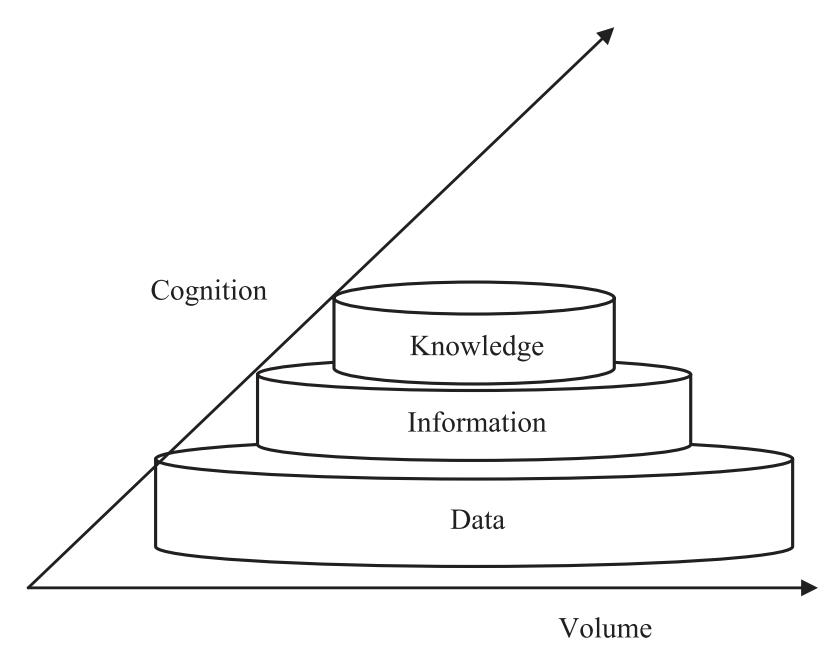
\includegraphics[scale=1.3]{se-wa-jpg/wissenprozess}
\caption[Wissensextraktion aus Daten]{Wissensextraktion aus Daten\protect\footnotemark}
\label{wissenprozess}
\end{figure}
\footnotetext{Vgl. Abbildung \textit{Shi} et al., Intelligent Knowledge, 2015, S. 5.}

\textit{Daten} stellen dabei nur eine Reihe von Zeichen dar, wobei deren Bedeutung zunächst unklar ist. Erst wenn bekannt wird, in welchem Kontext die Daten stehen und welche Beziehungen zwischen diesen bestehen, können diese interpretiert werden und zu einer (relevanten) \textit{Information} heranwachsen. Das \textit{Wissen} entsteht letztlich durch die Verknüpfung von den vielen Daten und Informationen, sowie den damit gesammelten Erfahrungen.\seFootcite{Vgl.}{S. 16-18}{Shi.2015}

Durch den Einsatz von modernster Computerhard- als auch Software ist es möglich, sehr große Datenmengen zu erheben, zu verarbeiten und zu analysieren, wodurch in diesem Kontext der Begriff \gls{bigdata} entstanden ist.\seFootcite{Vgl.}{S. 3}{Witten.2011} \gls{bigdata} bezeichnet Datenmengen, die mit herkömmlichen Analysemethoden nicht mehr zu verarbeiten sind und deshalb die Anwendung des Data Minings benötigen.\seFootcite{Vgl.}{S. 5}{Fasel.2016}\seFootcite{Vgl.}{S. 1}{Shi.2015} Hierzu einige ausgewählte Beispiele aus verschiedenen Datenbereichsquellen:\seFootcite{Vgl.}{S. 2}{Aggarwal.2015}

\begin{itemize}
\item \textbf{World Wide Web:} Die Anzahl der Dokumente im Internet hat seit langem die Milliarden-Marke geknackt, wobei die des unsichtbaren \glqq Webs\grqq~noch viel größer ist. Durch Nutzerzugriffe auf Inhalte, werden auf Serverseite Log-Dateien kreiert, um beispielsweise die Auslastung und Zugangszeiten zu protokollieren. Andererseits wird das Kundenverhalten auf kommerziellen Seiten aufgezeichnet, um personalisierte Werbung schalten zu können.

\item \textbf{Benutzerinteraktion:} Festnetzanbieter nutzen die durch Telefonate entstandenen Daten wie Gesprächslänge und -ort, um relevante Muster über die Netzwerksauslastung, zielgerichtete Werbung oder auch anzusetzende Preise durch Datenanalyse zu extrahieren.
\item \textbf{Internet of Things:} Durch kostengünstige (tragbare) Sensoren und deren kommunikative Vernetzung, entstand das \gls{iot}. Einer der Trends der heutigen Informationstechnologie, welcher durch die Erhebung von Massendaten eine signifikante Rolle für das Data Mining einnimmt.

\item \textbf{Weitere Beispiele:}  Social Media Plattformen (allen voran Facebook, Twitter und Co.), Finanzmärkte (z.B. der Aktienmarkt), Sport (z.B. Baseball, Basketball, Football oder wie in dieser Arbeit Fußball), uvm.\seFootcite{Vgl.}{S. 39}{Fayyad.1996}\seFootcite{Vgl.}{S. 1-2}{Han.2012}\seFootcite{Vgl.}{S. 85 ff}{Chu.2014} 
\end{itemize}

\glqq Wir befinden uns in einer Welt, in der wir reich an Daten sind, jedoch arm an Informationen und Wissen.\grqq\seFootcite{}{S. 5}{Han.2012} Der unglaublich rapide und enorme Datenzuwachs hat bei Weitem unsere menschliche Vorstellungskraft und Möglichkeiten übertroffen, sodass wir auf effiziente Werkzeuge angewiesen sind (siehe \vref{dmmethoden}). Die sich immer weiter ausbreitende Lücke zwischen Daten und Informationen, führt ausschließlich durch die Anwendung von Methoden des Data Minings zu den begehrten \glqq \textit{Golden Nuggets of Knowledge}\grqq.\seFootcite{Vgl.}{S. 5}{Han.2012} Dazu müssen die (Roh-)Daten gezielt ausgewählt und umstrukturiert werden, um diese anschließend durch Algorithmen analysieren zu können. Folglich entstanden Data Mining Prozesse, die dieses Problem mit Hilfe systematischer Abläufe lösen sollen (vgl. \vref{prozdm}). Zudem wird \glqq Data Mining [...] heute durch eine zunehmende Anzahl von Software-Tools unterstützt. Dazu zählen unter anderem Software-Lösungen wie: KNIME, MATLAB, SPSS, SAS, STATISTICA, TIBCO Spotfire, R, Rapid Miner, Tableau, QlikView, oder WEKA.\grqq\seFootcite{}{S. 3}{Runkler.2015} Das Software-Tool \textit{MATLAB} wird innerhalb der Funktionsmodellierung in \vref{fm} vorgestellt und anschließend als Werkzeug zur Anwendung von Data Mining Methoden in der Umsetzungsphase genutzt (vgl. \vref{umsetzung}).


\subsection{Data Mining Prozesse}
\label{prozdm}

In der Literatur grenzen viele Wissenschaftler den Begriff des eigentlichen Data Minings, vom Gesamtprozess der Extraktion von Wissen ab. Andere wiederum behandeln beide Termini synonym zueinander.\seFootcite{Vgl.}{S. 39}{Fayyad.1996}\seFootcite{Vgl.}{S. 2}{Mariscal.2010}\seFootcite{Vgl.}{S. 1}{Garcia.2015} Schlechte Qualität der Daten mindert die Leistungsfähigkeit des Data Minings. Um die Aussagekraft der Daten nicht zu gefährden, sind vorab Prozessschritte notwendig, die die Daten in adaptierter Form für die Methoden des Data Minings bereitstellen.\seFootcite{Vgl.}{S. 10}{Garcia.2015} Hierzu werden im Folgenden kurz die zwei bekanntesten Prozessmodelle vorgestellt:

\begin{itemize}
\item \gls{kdd}
\item \gls{crisp-dm}
\end{itemize}

\subsubsection{Knowledge Discovery in Data}
\label{dmkdd}

Der Begriff des \textit{Knowledge-Discovery-in-Data}-Prozesses wurde in den frühen 90er-Jahren geprägt und wird als \glqq nicht trivialer Prozess zur Identifizierung von gültigen, neuartigen, potentiell sinnvollen und letztlich verständlichen Mustern in Daten\grqq\seFootcite{}{S. 41}{Fayyad.1996} definiert.\seFootcite{Vgl.}{S. 2}{Mariscal.2010} Erstmals wurde der Terminus von Gregory Piatetsky-Shapiro auf der \textit{International Joint Conference on Artificial Intelligence}, 1989 in Detroit (USA), der Öffentlichkeit präsentiert.\seFootcite{Vgl.}{S. 1}{Adhikari.2015} Der in \vref{kddpic} dargestellte iterative \gls{kdd}-Prozess nach Fayyad, beinhaltet folgende Schritte, wobei das \gls{dm} als ein eigener Prozessschritt ausgewiesen wird:\seFootcite{Vgl.}{S. 5}{Cleve.2014}

\begin{enumerate}

\item \textbf{Datenselektion}: Auswahl der geeigneten Datenmengen.
\item \textbf{Datenvorverarbeitung}: Behandlung fehlender oder problembehafteter Daten.
\item \textbf{Datentransformation}: Umwandlung in adäquate Datenformate.
\item \textbf{Data Mining}: Suche nach Mustern.
\item \textbf{Interpretation und Evaluation}: Interpretation der Ergebnisse und Auswertung dieser.

\end{enumerate}

Auf die einzelnen Prozessschritte und deren Methoden wird genauer in \vref{kdd} eingegangen. Die Abkürzung \textit{KDD} steht in der Literatur für unterschiedliche Bezeichnungen, wie zum Beispiel \textit{Knowledge Discovery in Databases}, \textit{Knowledge Discovery in Data Mining} oder \textit{Knowledge Discovery in Data Warehouses}.\seFootcite{Vgl.}{S. 26 ff}{OseiBryson.2015} Alle zielen dabei auf die Erforschung von Wissen aus Datenmengen ab, wofür in dieser Arbeit die allgemeingültige Bezeichnung \textit{Knowledge Discovery in Data} verwendet wird.

\begin{figure}[H]
\centering
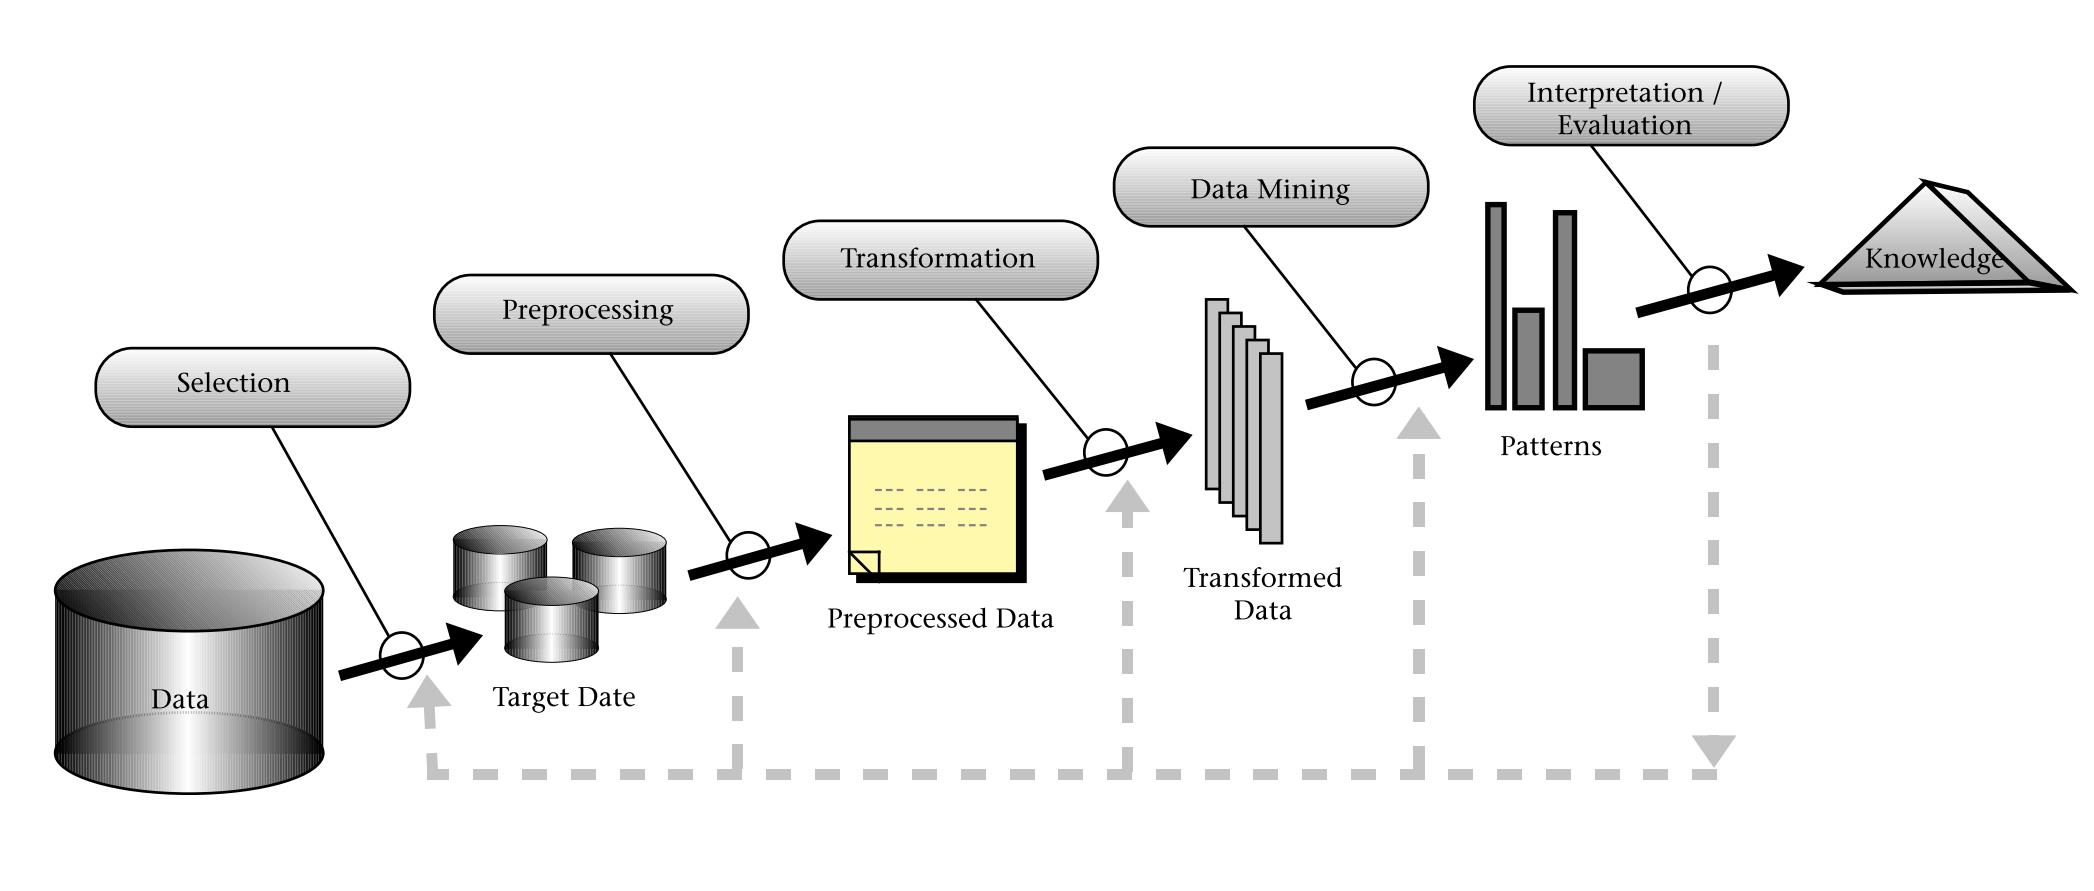
\includegraphics[scale=0.85]{se-wa-jpg/kdd}
\caption[Der Knowledge Discovery in Data Prozess]{Der Knowledge Discovery in Data Prozess\protect\footnotemark}
\label{kddpic}
\end{figure}
\footnotetext{Vgl. Abbildung \textit{Fayyad} et al., From Data Mining to Knowledge, 1996, S. 41.}


\subsubsection{CRISP-DM}
Das \gls{crisp-dm}-Modell wurde im Jahr 2000 durch ein Konsortium, bestehend aus mehreren nachfolgenden aufgeführten Firmen, entwickelt.\seFootcite{Vgl.}{S. 6}{Cleve.2014}\seFootcite{Vgl.}{S. 3}{Mariscal.2010}

\begin{itemize}
\item NRC Corporation
\item Daimler AG
\item SPSS Inc.
\item Teradata 
\item OHRA
\end{itemize}

Dieses Modell verfolgt das Ziel, einen standardisierten und branchenübergreifenden Data-Mining-Prozess zu definieren und das dadurch berechnete Modell zu validieren. Hierbei wird von einem Lebenszyklus, bestehend aus sechs Etappen, ausgegangen, der in \vref{crisp} dargestellt wird.\seFootcite{Vgl.}{S. 6-8}{Cleve.2014} Im Folgenden werden dazu die einzelnen Schritte des Prozesses aus der Abbildung (nummeriert von Schritt 1 bis 6) kurz erläutert.

\begin{figure}[H]
\centering
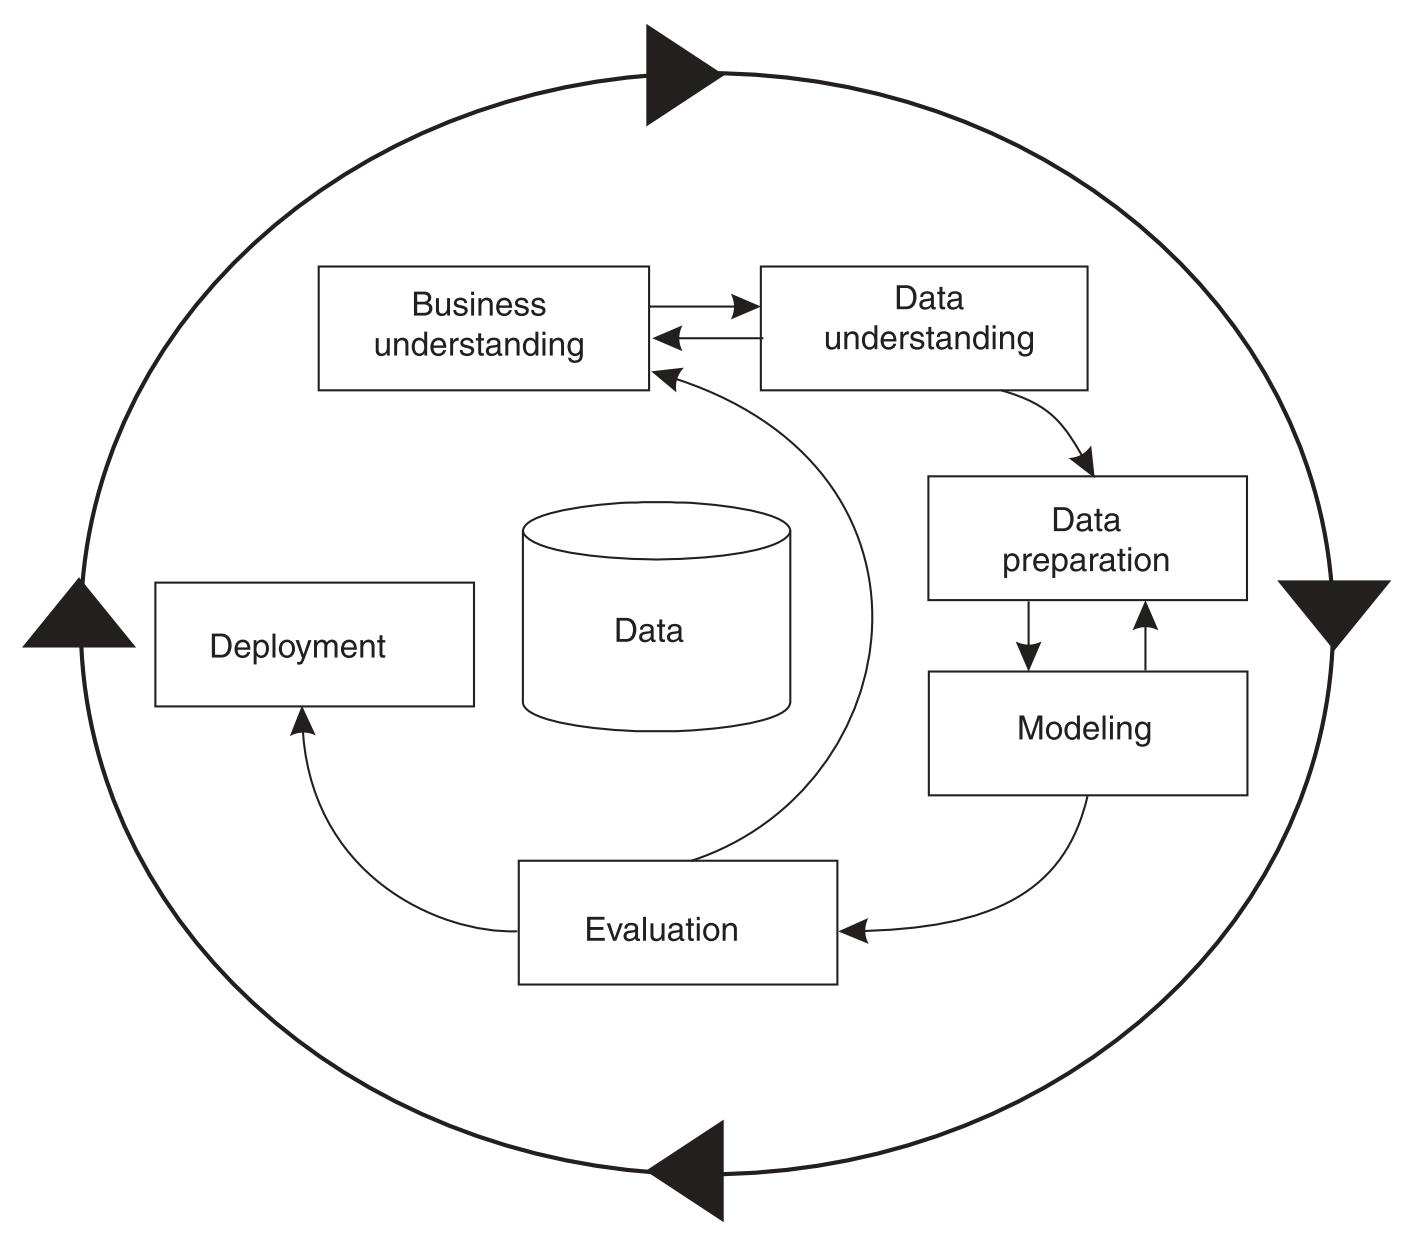
\includegraphics[scale=0.9]{se-wa-jpg/crisp}
\caption[CRISP-DM Prozess]{CRISP-DM Prozess\protect\footnotemark}
\label{crisp}
\end{figure}
\footnotetext{Vgl. Abbildung \textit{Mariscal} et al., A survey of data mining, 2010, S. 13}

\paragraph{1. Verstehen der Aufgabe}(\textit{Business understanding}): 
Hier steht das grundsätzliche Verständnis des Fachgebietes und der Aufgabe im Vordergrund. Die Ziele werden definiert, Ressourcen des Unternehmens ermittelt und die Ausgangssituation bestimmt. Weiterhin müssen Erfolgskriterien quantifiziert und Risiken eruiert werden, um eine Kostenplanung aufstellen zu können. 
\paragraph{2. Verständnis der Daten}(\textit{Data understanding}): 
Diese Phase beschäftigt sich mit den benötigten Daten zur Durchführung der Analyse. Daten werden gesammelt und beschrieben, um deren betrieblichen Kontext, indem sie stehen, zu verstehen.
\paragraph{3. Datenvorbereitung}(\textit{Data preparation}): 
Es gilt den Data-Mining-Prozess-Schritt vorzubereiten, wobei fehlerhafte und inkonsistente Daten korrigiert werden müssen, um diese schließlich in eine Datenstruktur transformieren zu können, die für die Methoden des Data Minings nutzbar sind.
\paragraph{4. Data Mining - Modellbildung}(\textit{Modeling}): 
In dieser Phase wird ein Modell mit Hilfe des Data Minings erstellt, welches durch einen iterativen Aufbau immer wieder verfeinert und verbessert wird. 
\paragraph{5. Evaluation:}
Die erzielten Ergebnisse werden an den aus Phase 1 definierten Erfolgskriterien gemessen, um festzustellen, ob der wirtschaftliche Nutzen erzielt wird.
\paragraph{6. Einsatz im Unternehmen}(\textit{Deployment}): 
Zuletzt gilt es, den Einsatz der Resultate im Unternehmen vorzubereiten und diese in das operative Geschäft zu integrieren.

Das Modell bezieht und orientiert sich, wie schon am Namen zu erkennen ist, stark an wirtschaftlichen Projekten und beschreibt \textit{Was} zu tun ist, jedoch nicht genau \textit{Wie}, sodass Projektteams innerhalb dieses Rahmens damit beginnen ihre eigenen Methoden zu entwickeln.\seFootcite{Vgl.}{S. 4}{Mariscal.2010}

Im Vergleich zum \gls{kdd}-Modell nach Fayyad, sind die Phasen 1 und 2 des \gls{crisp-dm}-Modells sehr stark projektabhängig und spiegeln die Sicht der Industrie auf das Projekt wider.\seFootcite{Vgl.}{S. 8}{Cleve.2014} Im Gegensatz dazu konzentriert sich der \gls{kdd}-Prozess auf die Datenbereitstellung und Analyse, sodass dieser als grundlegende Methodik für die spätere Umsetzung der wissenschaftlichen Aufgabenstellung herangezogen wird und genauer in \vref{kdd} beleuchtet wird.

Mariscal et al. diskutieren in ihrer Studie zahlreiche weitere Prozessmodelle zur Extraktion von Wissen aus riesigen Datenmengen, wobei die Kernelemente der Datenselektion, -vorverarbeitung und -tranformation, sowie der anschließende Schritt des eigentlichen Data Minings immer wieder aufzufinden sind.\seFootcite{Vgl. vorgestellte Modelle aus}{}{Mariscal.2010} Nicht zuletzt ist zu erwähnen, dass in der Literatur unterschiedliche Auffassungen zu dem Begriff des Data Minings existieren und dieser oftmals mit den Data Mining Prozessen synonym verwendet wird. Ein Hinweis darauf sind auch die weit über 500 wissenschaftlichen Artikel zu dem Journal \textit{Data Mining and Knowledge Discovery} auf \textit{Springer Link}.



\section{Knowledge Discovery in Data}
\label{kdd}

Das folgende Kapitel beschreibt den \textit{Knowledge-Discovery-in-Data}-Prozess, der im vorherigen Kapitel (vgl. \vref{dmkdd}) als grundlegende Methodik der Arbeit ausgewählt wurde. Hierzu werden die einzelnen Prozessschritte der Datenselektion, der Datenvorverarbeitung, der Datentransformation, der Data-Mining-Methoden, sowie der Interpretation der Ergebnisse konkretisiert, um diese in der späteren Umsetzung der wissenschaftlichen Aufgabe anwenden zu können.

\glqq Experten [...] haben realisiert, dass eine große Anzahl an Datenquellen der Schlüssel zu bedeutsamen Wissen sein kann und das dieses Wissen in dem Entscheidungsfindungsprozess genutzt werden sollte. Eine einfache \gls{sql}-Abfrage oder \gls{olap} reichen für eine komplexe Datenanalyse oft nicht aus.\grqq\seFootcite{}{S. 1}{Adhikari.2015} Hier greift der in \vref{kddpic} dargestellte \gls{kdd}-Prozess, ein multiples iteratives Modell, in dem die einzelnen Schritte solange wiederholt und aufeinander abgestimmt werden müssen, bis aus den zugrundeliegenden Daten, Wissen abgeleitet werden kann.\seFootcite{Vgl.}{S. 7}{Mariscal.2010} Das Data Mining selbst kommt erst nach ausführlicher Datenvorbereitung zum Einsatz und kann so zu einer automatischen und explorativen Anpassung eines Modells -- wie bei der Funktionsmodellierung (vgl. \vref{fm}) -- an riesige Datenmengen genutzt werden.\seFootcite{Vgl.}{S. 1}{Adhikari.2015}\seFootcite{Vgl.}{S. 7}{Mariscal.2010}

In der Literatur existieren unterschiedliche Vorstellungen der einzelnen Prozessschritte, wodurch es oftmals zu Überschneidungen zwischen den einzelnen Gebieten kommt. So findet sich die Methode der \textit{Data Integration} einerseits in der Datenselektion wieder, andererseits auch in der Datenvorverarbeitung.\seFootcite{Vgl.}{S. 1}{Garcia.2015}\seFootcite{Vgl.}{S. 198}{Cleve.2014} Im Folgenden wird versucht, diese Schritte klar voneinander abzutrennen. Hierbei wird sich größtenteils an den Ausarbeitungen von Han et al. und Cleve et al. orientiert.



\section{Datenselektion}
\subsection{Datenvorverarbeitung}
\label{aufbereitung}
\glqq Da die Zieldaten aus den Datenquellen lediglich extrahiert werden, ist im Rahmen der Datenvorverarbeitung die Qualität des Zieldatenbestandes zu untersuchen und – sofern nötig – dieser durch den Einsatz geeigneter Verfahren zu verbessern.\grqq\seFootcite{}{S. 9}{Cleve.2014}

Diese essentielle Phase verfolgt das Ziel, die unstrukturierten und zunächst nutzlos scheinenden, selektierten Rohdaten, in qualitativ hochwertigere Daten umzuwandeln, um diese der passenden \gls{dm}-Methode in einem geeigneten Format bereitstellen zu können. Die Struktur und das Format müssen perfekt auf die vorliegende Aufgabe passen, ansonsten führt die geringe Qualität der Daten zu schlechten bzw. falschen Resultaten, bis hin zu Laufzeitfehlern.\seFootcite{Vgl.}{S. 10-11}{Garcia.2015} Es gilt auch hier das Prinzip: GIGO – garbage in, garbage out.\seFootcite{Vgl.}{S. 197}{Cleve.2014} Die oftmals schlechte Qualität der (Roh-)Daten ist durch \textit{fehlende, ungenaue, inkonsistente bzw. widersprüchliche} Daten zu begründen.\seFootcite{Vgl.}{S. 84}{Han.2012}\seFootcite{Vgl.}{S. 196}{Cleve.2014} Im Folgenden werden dazu einige Ursachen beispielhaft aufgeführt.

Ungenaue bzw. falsche Daten können schon bei der Erhebung entstehen, wenn ein falsches Datenerhebungsinstrument ausgewählt wird. Bei Stichproben sollte die Gesamtmenge so präzise wie möglich widergespiegelt werden, um die Datenakkuratesse nicht zu gefährden.\seFootcite{Vgl.}{S. 25}{Fahrmeir.2007} Weiterhin können technische und menschliche Fehler zu ungenauen Daten führen, indem Personen beispielsweise ihre persönlichen Informationen bei einer Befragung absichtlich verschleiern (z.B. Standardwert für Geburtsdatum 1. Januar), wobei man diese Problematik auch als \textit{\glqq disguised missing data\grqq}~bezeichnet.\seFootcite{Vgl.}{S. 84}{Han.2012}\seFootcite{Vgl.}{S. 24}{Fahrmeir.2007}\seFootcite{Vgl.}{S. 196}{Cleve.2014} Neben der falschen subjektiven Einschätzung des Menschen bei der Erhebung, können auch von einem technischem Blickwinkel ungenaue Daten ermittelt werden, wie z.B. durch (teils-)defekte Sensoren.\enlargethispage{\baselineskip}  Nicht zuletzt können Daten bei einem Transfer verfälscht werden bzw. sogar verloren gehen.\seFootcite{Vgl.}{S. 84}{Han.2012}

Fehlende Daten lassen sich einerseits durch technische Mängel begründen, andererseits auch durch die Tatsache, dass bestimmte Attribute schlichtweg von Beginn an bei der Erhebung nicht beachtet wurden oder durch bestimmte Restriktionen nicht verfügbar waren.\seFootcite{Vgl.}{S. 84-85}{Han.2012}

Die aufgezeigten Beispiele spiegeln nur einen kleinen Teil möglicher Ursachen wider und sollen die Bedeutsamkeit dieser Phase für den Data-Mining-Prozess aufzeigen. Die Datenvorbereitung stellt dabei einige leistungsstarke Werkzeuge zur Verfügung, um die Datenqualität nachhaltig zu verbessern:\seFootcite{Vgl.}{S. 11 ff}{Garcia.2015}\seFootcite{Vgl.}{S. 196 ff}{Cleve.2014}\seFootcite{Vgl.}{S. 84 ff}{Han.2012}

\begin{itemize}
\item \textbf{Data Cleaning}: In diesem Schritt werden die Daten bereinigt, indem beispielsweise \textit{fehlerhafte} oder \textit{störende} Daten korrigiert werden (siehe \vref{dc}).

\item \textbf{Data Integration}: Diese Phase beschäftigt sich mit der fehlerfreien Zusammenführung von Daten, da diese oftmals aus mehreren unterschiedlichen Quellen stammen (siehe \vref{di}).

\item \textbf{Data Reduction}: Um die Algorithmen der Data Mining Methoden nutzen zu können, muss die exorbitante Datenmenge reduziert bzw. komprimiert werden, sodass lange Laufzeiten verhindert beziehungsweise reduziert werden können (siehe \vref{dr}).
\end{itemize}

Auf die in \vref{werkzeuge} vereinfacht dargestellten Werkzeuge und ihre Konzepte, wird in den folgenden Unterkapiteln näher eingegangen.

\begin{figure}[H]
\centering
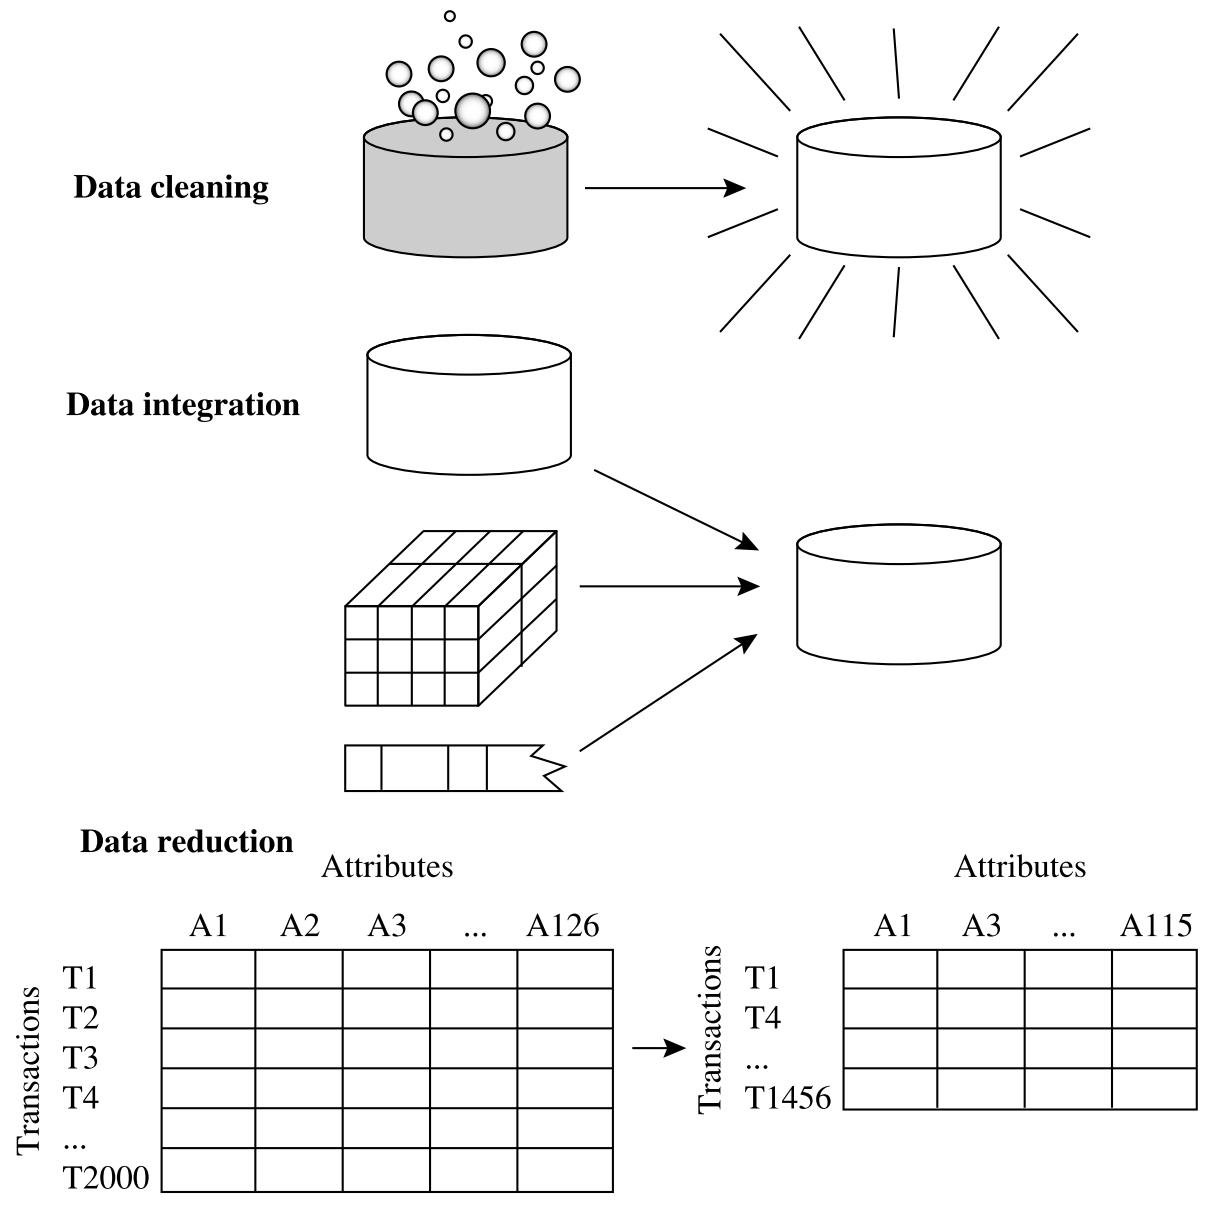
\includegraphics[scale=1.2]{se-wa-jpg/preprocessing}
\caption[Werkzeuge der Datenvorverarbeitung]{Werkzeuge der Datenvorverarbeitung\protect\footnotemark}
\label{werkzeuge}
\end{figure}
\footnotetext{Vgl. Abbildung \textit{Han}, Data Mining: Concepts and techniques, 2012, S. 87}


\subsubsection{Data Cleaning}
\label{dc}
In der realen Welt sind Daten häufig \glqq unvollständig, mit Fehlern oder Ausreißern behaftet oder sogar inkonsistent.\grqq\seFootcite{}{S. 199}{Cleve.2014} Um Fehler oder gar falsche Resultate im Data-Mining-Prozess frühzeitig zu vermeiden, ist es von großer Bedeutung, die Datenmengen zu bereinigen. Der Fokus sollte hierbei auf der Informationsneutralität liegen. Das bedeutet, es sollen möglichst keine neuen Informationen hinzugefügt werden, die das reale Abbild verzerren oder verfälschen können.\seFootcite{Vgl.}{S. 199-200}{Cleve.2014} Folgende Problemarten gilt es zu behandeln:

\paragraph{Fehlende Daten} 
Dem Datenanalyst stehen einige Möglichkeiten zur Verfügung, um auf fehlende Daten zu reagieren:\seFootcite{Vgl.}{S. 88-90}{Han.2012}\seFootcite{Vgl.}{S. 200-201}{Cleve.2014}

\begin{itemize}
\item \textit{Attribut ignorieren}
\\ Der Datensatz mit dem fehlenden Attribut wird gänzlich ignoriert oder gelöscht. Jedoch können dadurch wichtige Informationen für die Datenanalyse verloren gehen, wodurch dieses Verfahren nur bei Datensätzen mit mehreren Lücken angewandt werden sollte.

\item \textit{Manuelles Einfügen}
\\ Besitzt der Datenanalyst das nötige Wissen, kann dieser einzelne Datensätze nachträglich manuell einfügen. Dieser Vorgang entwickelt sich schnell zu einem sehr zeitaufwändigen und schwer zu realisierenden Vorgang, der aufgrund des Mangels an Ressourcen (personeller wie auch zeitlicher) nicht zu realisieren ist, sobald die Datenmenge wächst (z.B. Nachtrag von 500 Kundendaten per Hand).

\item \textit{Globale Konstante}
\\ Den fehlenden Wert durch eine globale Konstante (auch als Standardwert bezeichnet) zu ersetzen, ist sinnvoll, wenn auch ein leeres Feld als Information angesehen wird. Beispiele für Konstanten wären \textit{unbekannt} oder \textit{minus unendlich}.

\item \textit{Durchschnittswert}
\\ Handelt es sich bei dem fehlenden Attribut um einen metrischen Wert, so kann der Durchschnittswert aller Einträge als Ersatz verwendet werden. Der Durchschnittswert bietet sich als äußerst einfache Möglichkeit, wenn die Daten klassifiziert werden können und die Berechnung nur auf Datensätzen der selben Klasse angewandt wird. Die Methode der \gls{knn}\seFootcite{Vgl.}{S. 76}{Garcia.2015} steht zur Verfügung, wenn keine Klassen vorhanden sind. Hierbei wird der Durchschnitt, der dem aktuellen Datensatz ähnlichsten Werte benutzt.

\item \textit{Wahrscheinlichster oder häufigster Wert}
\\ Durch statistische Methoden kann der wahrscheinlichste Wert für das fehlende Attribut ermittelt werden, jedoch sollte diese Angleichung begründet sein. Bei nicht numerischen Werten kann als weitere Möglichkeit auch der häufigste Wert als Ersatz für das fehlende Attribut verwendet werden.
\end{itemize}

\paragraph{Verrauschte Daten und Ausreißer}
\label{outlierchapter}
Durch ungenaue Messwerte oder falsche Schätzungen entstehen die sogenannten \textit{verrauschten Daten}.\footnote{Im englischen Sprachgebrauch als \textit{noisy data} bekannt.} Um diese bereinigen zu können, stehen dem Datenanalyst einige Verfahren zur Verfügung, durch welche diese fehlerbehafteten Daten angeglichen werden können.\footnote{Auch als \textit{smoothing} bekannt.} Als \textit{Ausreißer} bezeichnet man dabei Daten, die erheblich von den anderen Daten abweichen oder außerhalb eines Wertebereiches (z.B. $0<x<100$) liegen.\seFootcite{Vgl.}{S. 89-90}{Han.2012} Beispielsweise liegen bei einer Befragung Daten von 30- bis 50-Jährigen vor, darunter auch einer von einem 90-Jährigen, könnte es sich hierbei um einen Ausreißer handeln, aber auch um einen fehlerhaften Datensatz.\seFootcite{Vgl.}{S. 196}{Cleve.2014} \glqq Ob solche Ausreißer für das Data Mining ausgeblendet oder adaptiert werden sollten oder besser doch im Originalzustand zu verwenden sind, hängt vom konkreten Kontext ab.\grqq\seFootcite{}{S. 196}{Cleve.2014}


\begin{itemize}

\item \textit{Klasseneinteilung (bining)}
\\ Durch die Gruppierung verrauschter Daten in Klassen, können diese beispielsweise durch den Mittelwert oder die naheliegenden Grenzwerte ersetzt werden. 

\item \gls{regression}
\\ Die Darstellung der Daten in Form einer mathematischen Funktion, bietet die Möglichkeit, fehlerbehaftete Daten  durch die berechneten Funktionswerte zu ersetzen. Für zwei Abhängigkeiten zwischen zwei Attributen steht hierbei neben der \textit{linearen Regression}, auch die \textit{multiple lineare Regression} für mehrere Attribute als Werkzeuge zur Verfügung (weiterführende Ausarbeitung zur Regressionsanalyse siehe \vref{ra}). 

\item \textit{Verbundbildung (clustering)}
\\ Eine der einfachsten Möglichkeiten um Ausreißer zu erkennen, bietet die Verbundbildung, auch \gls{clustering} genannt. Hierbei werden ähnliche Daten, wie in \vref{outlier} dargestellt, zu \textit{Clustern} zusammengeführt, wodurch sich die Ausreißer direkt identifizieren lassen.

\begin{figure}[H]
\centering
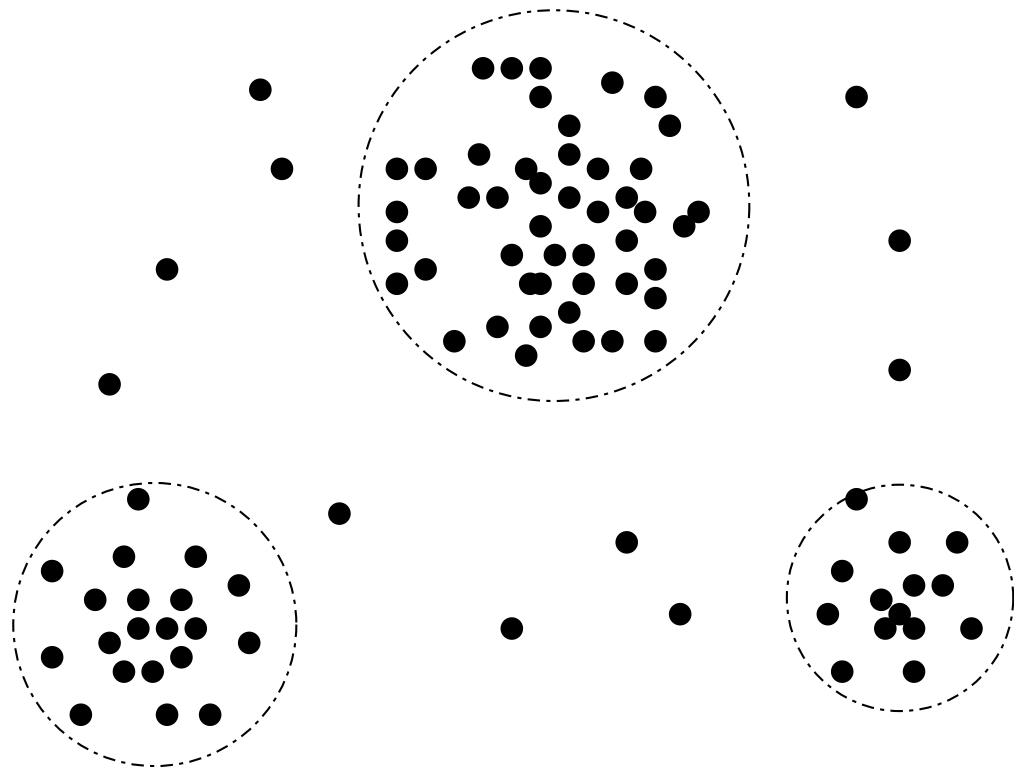
\includegraphics[scale=1.2]{se-wa-jpg/outlier}
\caption[Outlierdetection mittels Clustering]{Outlierdetection mittels Clustering\protect\footnotemark}
\label{outlier}
\end{figure}
\footnotetext{Vgl. Abbildung \textit{Han}, Data Mining: Concepts and techniques, 2012, S. 91}
\end{itemize}

\paragraph{Falsche und inkonsistente Daten}
Bei falschen bzw. inkonsistenten Daten ergeben sich prinzipiell zwei Möglichkeiten zur Korrekturbehandlung. Einerseits können der Datensatz oder bestimmte Attribute durch \textit{Löschen} entfernt werden, wobei jedoch die Gefahr einer zu großen Reduktion des Datenbestandes entsteht und relevante Informationen für das Data Mining verloren gehen könnten. Die zweite Korrekturvariante versucht den inkonsistenten Datensatz, durch die \textit{Zuhilfenahme anderer Datensätze}, sinnvoll zu ersetzen. Sollte eine Unterscheidung zwischen \textit{falsch} und \textit{richtig} nicht möglich sein, wären beim Löschen immer mindestens zwei Datensätze betroffen.\seFootcite{Vgl.}{S. 203-204}{Cleve.2014}

\subsubsection{Data Integration}
\label{di}
Bei Data-Mining-Projekten ist oftmals die Integration mehrerer Datenbestände aus unterschiedlichen Quellen erforderlich. Diese Phase sollte mit äußerster Sorgfalt durchgeführt werden, um frühzeitig redundante und inkonsistente Datensätze zu vermeiden, wodurch die Genauigkeit und Geschwindigkeit der nachfolgenden Data Mining Algorithmen nicht gefährdet wird.\seFootcite{Vgl.}{S. 93-94}{Han.2012} Folgende Punkte gilt es bei der Datenintegration zu beachten:

\begin{itemize}
\item \textbf{Identifikationsproblem von Entitäten}:
\\ Bei der Datenintegration aus multiplen Datenquellen, wie beispielsweise Datenbanken oder Dokumenten, stellt die Schema-Integration wie auch die Objektanpassungen eine schwierige Herausforderung dar. Der Datenanalyst muss sicherstellen, dass zum Beispiel das Attribut \textit{kunden\_nummer} aus der einen Datenquelle, die selbe Referenz besitzt, wie das Attribut \textit{kunden\_id} aus einer anderen und es sich folglich um das selbe Attribut handelt. Dies wird allgemein als \textit{Problem Identification Problem} bezeichnet.\seFootcite{Vgl.}{S. 199}{Cleve.2014}\seFootcite{Vgl.}{S. 94}{Han.2012} Die Metadaten der Attribute beinhalten Informationen, wie \textit{Name, Bedeutung, Datentyp, Wertebereich, uvm.} und können durch Abgleich derer zu einer Vermeidung von Fehlern bei der Integration beitragen. Weiterhin muss gesondert auf die \textit{Datenstruktur} geachtet werden, um keine referentiellen Abhängigkeiten bzw. Beziehungen zwischen den Daten zu zerstören.\seFootcite{Vgl.}{S. 94}{Han.2012} 

\item \textbf{Redundanzen bei Attributen}:
\\ Ein Attribut, welches durch ein anderes Attribut ableitbar ist -- wie zum Beispiel das Alter vom Geburtsjahr berechnet werden kann -- wird als redundant bezeichnet. Die Vielzahl von Redundanzen führt zu unnötig großen Datenmengen, die wiederum die Performanz sowie die Resultate eines Data Mining Algorithmus negativ beeinträchtigen können.\seFootcite{Vgl.}{S.41}{Garcia.2015} Folglich sollte diese Problematik durch die Anwendung von statistischen Verfahren, in Form der Korrelationsanalyse, dezidiert behandelt werden. Für numerische Werte ist dabei der Einsatz von Korrelationskoeffizienten und Kovarianzen hilfreich. Um die Implikation zweier Attribute einer nominalen Datenmenge\footnote{Rein qualitative Merkmalsausprägungen ohne natürliche Rangordnung (wie z.B. das Geschlecht).} bestimmen zu können, verwendet man in der Regel den $\chi^2$(\textit{Chi-Quadrate})-Test.\seFootcite{Vgl.}{S. 95.}{Han.2012}\seFootcite{Vgl.}{S. 41}{Garcia.2015}\seFootcite{Vgl.}{S. 64}{Cleve.2014} 

\item \textbf{Duplikatserkennung}:
\\ Duplikate verkörpern Redundanzen auf Datensatzebene und führen einerseits zu unnötig großen Datenmengen, die sich wiederum auf die Performanz der Algorithmen auswirken. Andererseits führt jedoch auch die verfälschte Gewichtung der mehrfach vorkommenden Datensätze, zu falschen Analyseergebnissen. Ein häufiger Grund stellt dabei die Verwendung von denormalisierten Datenbanktabellen dar.\seFootcite{Vgl.}{S. 98}{Han.2012}\seFootcite{Vgl.}{S. 43}{Garcia.2015}

\item \textbf{Konflikte bei Attributswerten}:
\\ Hierbei handelt es sich um die unterschiedliche Darstellung, Skalierung und Kodierung von Attributswerten. Beispielsweise kann das Attribut \textit{Gewicht} durch das metrische System oder das britische Maßsystem repräsentiert werden, woraus bei der Zusammenführung von Daten in eine einheitliche Quelle immer wieder Konflikten resultieren.\seFootcite{Vgl.}{S. 99}{Han.2012}\seFootcite{Vgl.}{S. 199}{Cleve.2014} 
\end{itemize}

\subsubsection{Data Reduction}
\label{dr}
Die bereits mehrfach angesprochene Problematik der riesigen Datenmengen bei Data-Mining-Projekten, steigert die Komplexität und vermindert die Effizienz der Algorithmen. Daher strebt die Datenreduktion -- wie die Bezeichnung erkennen lässt -- nach einer reduzierten repräsentativen Teilmenge, welche die Integrität des Originals nicht verliert. Dazu können folgende drei Techniken angewandt werden:\seFootcite{Vgl.}{S. 147 ff}{Garcia.2015}\seFootcite{Vgl.}{S. 99-100}{Han.2012}\seFootcite{Vgl.}{S. 206-208}{Cleve.2014} 

\begin{enumerate}

\item Dimensionsreduktion 

\item Datenkompression

\item Numerische Datenreduktion

\end{enumerate}

\paragraph{Dimensionsreduktion}
Hierbei bleiben irrelevante Attribute des Datensatzes unberücksichtigt und nur für die Analyse relevante Daten werden miteinbezogen. Allgemein empfehlen sich dafür zwei Verfahren: Bei der schrittweisen \textit{Vorwärtsauswahl} werden wesentliche Attribute einer sukzessiv wachsenden Zielmenge zugeordnet. Im Gegensatz dazu werden bei der \textit{Rückwärtseliminierung} die uninteressanten Daten schrittweise aus der Zielmenge eliminiert.\seFootcite{Vgl.}{S. 206}{Cleve.2014} 

\paragraph{Datenkompression}
\label{datenkompression}
Bei dieser Technik wird durch Transformation oder Codierung versucht, eine Reduktion der Datenmenge zu erreichen. Fasst man beispielsweise die einzelnen Attribute \textit{Tag, Monat und Jahr} zu einem neuen Attribut \textit{Datum} zusammen, können Datensätze komprimiert werden.\seFootcite{Vgl.}{S. 207}{Cleve.2014}
 
\paragraph{Numerische Datenreduktion}
Statt die gesamte Datenmenge für die Analyse heranzuziehen, wird innerhalb der numerischen Datenreduktion eine repräsentative Teilmenge -- in Form einer Stichprobe -- für das \gls{dm} genutzt. Im Vordergrund steht hierbei die passende Auswahl unterschiedlicher Stichprobeverfahren, wie der \textit{zufälligen Stichprobe} oder der \textit{repräsentativen Stichprobe}, woraus jedoch kein verzerrtes Abbild der Daten resultieren darf.\seFootcite{Vgl.}{S. 25-27}{Fahrmeir.2007}\seFootcite{Vgl.}{S. 207}{Cleve.2014}
\subsection{Datentransformation}
\label{dt}
Nachdem die (Roh-)Daten selektiert, bereinigt und auf eine relevante Zielmenge reduziert wurden, müssen diese noch in eine adaptierte Form für die Algorithmen des Data Minings transformiert werden.\seFootcite{Vgl.}{S. 112}{Han.2012} Oftmals müssen sogar neue Attribute aus einem Datensatz kreiert werden, da dieser nicht in geeigneter Struktur für das Data-Mining-Verfahren vorliegt.\seFootcite{Vgl.}{S. 48}{Garcia.2015} Dazu gibt es eine Reihe an unterschiedlichen Transformationsmöglichkeiten, wobei in dieser Arbeit ein Auszug der relevanten Methoden vorgestellt werden soll:

\paragraph{Codierung}
Liegen beispielsweise Attribute mit einer ordinalen Ausprägung vor (wie \textit{sehr groß, groß, mittel und klein}), müssen diese bei einer Verwendung des \gls{knn}-Algorithmus in numerische Werte transformiert werden (Werte zwischen 0 und 1). Hierbei würde sich folgende Codierung für das Attribut \textit{Körpergröße} anbieten:\seFootcite{Vgl.}{S. 210}{Cleve.2014}

\begin{itemize}
\item \textit{sehr groß} $\rightarrow$ 1
\item \textit{groß} $\rightarrow$ 0,66
\item \textit{mittel} $\rightarrow$ 0,33
\item \textit{klein} $\rightarrow$ 0
\end{itemize}

Die Ordnungsrelation, hier \textit{sehr groß > groß > ...}, darf dabei jedoch nicht verloren gehen. In Abhängigkeit zu dem jeweiligen Verfahren, müssen Daten, so wie dies bei Maßeinheiten immer wieder der Fall ist, oftmals kodiert werden.\seFootcite{Vgl.}{S. 211}{Cleve.2014}

\paragraph{Normalisierung und Skalierung}
Unterschiedliche Maßeinheiten -- wie \textit{Körpergröße} und \textit{Körpergewicht} -- können die Datenanalyse negativ beeinflussen und müssen daher in eine einheitliche Skalierung transformiert werden, um eine gleiche Gewichtung aller Attribute zu erreichen. Man bedient sich hierbei in der Regel an der \textit{Min-Max-Normalisierung} (siehe \vref{minmax}) oder der \textit{Z-Transformation}, um numerische Werte auf ein [0,1] Intervall zu normieren.\seFootcite{Vgl.}{S. 114}{Han.2012}\seFootcite{Vgl.}{S. 212}{Cleve.2014}

\begin{figure}[H]
\begin{equation}
x_{neu} = \frac{x - min(x_i)}{max(x_i) - min(x_i)}
\end{equation}
\caption{Min-Max-Normalisierung}
\label{minmax}
\end{figure}

\paragraph{Datenaggregation}
Nicht nur aus Sicht der Datenkompression (vgl. \vref{datenkompression}) ist die Datenaggregation erforderlich. Vielmehr \glqq kann die Aggregation aus inhaltlichen Gründen sinnvoll sein.\grqq\seFootcite{}{S. 214}{Cleve.2014} Wenn Daten auf einer zu detaillierten Ebene vorliegen -- wie beispielsweise Einwohnerzahlen von Stadtteilen -- müssen diese für einen Städtevergleich erst summiert werden, um bundesweite Aussagen treffen zu können. Je nach Kontext können verschiedene Aggregationsmethoden (wie z.B. Summenbildung, Durchschnitt, usw.) für die Transformation zu einem einzigen Wert angewendet werden.\seFootcite{Vgl.}{S. 112}{Han.2012}

\paragraph{Datenglättung}
Die bereits in \vref{outlierchapter} vorgestellten Techniken zur Bereinigung von verrauschten Daten und Ausreißern, finden auch bei der Transformation ihre Verwendung. Die Datenglättung strebt nach einer reduzierten Datenmenge, in welcher jeder numerische Wert durch einen idealisierten Wert, wie beispielsweise der \textit{\gls{regression}}, ersetzt wird.\seFootcite{Vgl.}{S. 214-215}{Cleve.2014}
\subsection{Data-Mining-Methoden}
\label{dmmethoden}

Nachdem die Daten in geeigneter Form vorliegen, kommt das eigentliche Herzstück des \gls{kdd}-Prozesses -- das \textit{Data Mining} -- zum Tragen. In diesem Schritt wird zu nächst überprüft, welche grundlegende Data-Mining-Aufgabe es zu lösen gilt, um anschließend ein passendes Analyseverfahren zur Identifizierung von Mustern und Zusammenhängen auswählen zu können.\seFootcite{Vgl.}{S. 10}{Cleve.2014} Die interdisziplinäre Wissenschaft des Data Minings umfasst bewährte Techniken aus mehreren Forschungsgebieten, welche auf verschiedenste Problemfälle der Realität, wie Zeitreihenanalysen, Funktionsmodellierungen, Klassifikation uvm., angewendet werden können. Grundsätzlich basieren fast alle Analyseverfahren auf der Mathematik, insbesondere der Statistik.\seFootcite{Vgl.}{S. 12}{Cleve.2014} Im Allgemeinen unterteilt man die Data-Mining-Methoden in zwei Kategorien: \textit{Prognose} und \textit{Beschreibung}. Hierzu gibt \vref{dmmethods} einen Überblick über die Einteilung der etablierten Methoden, welche im Folgenden kurz aufgeführt werden.

\paragraph{Prognose:} In dem Bereich der Prognose unterscheidet man zwischen zwei Gruppen: \textit{statistische Methoden} und \textit{symbolische Methoden}. Letztere versuchen das Wissen durch Symbolik und Verknüpfung, auf einer leichter interpretierbaren Ebene für Menschen, zu vermitteln. Im Gegensatz dazu, repräsentieren statistische Methoden das Wissen mit Hilfe der Erstellung von mathematischen Modellen.\seFootcite{Vgl.}{S. 3}{Garcia.2015} Die am häufigsten angewendeten statistischen Methoden sind folgende:\seFootcite{Vgl.}{S. 3-5}{Garcia.2015}\seFootcite{Vgl.}{S. 23-24}{Han.2012}

\begin{itemize}
\item \textit{Regressionsanalyse}
\\ Die älteste \gls{dm}-Methode dient zur Funktionsmodellierung von einer abhängigen oder mehreren unabhängigen Variablen. Die Form der Funktion wird dabei durch das ausgewählte Verfahren, beispielsweise \textit{lineare oder quadratische Regression}, bestimmt und kann anhand bestimmter Parameter validiert werden, wie \glqq gut\grqq~diese zu den eingebrachten Daten passt.\seFootcite{Vgl.}{S. 3}{Garcia.2015}

\item \textit{(Künstliche)} \gls{nn}
\\ In diesem Teilbereich der künstlichen Intelligenz wird versucht, einen Wissensspeicher zu kreieren, der ähnlich unserem leistungsfähigen Gehirn funktioniert. Hierbei werden die biologischen Elemente und Vorgehensweise des Gehirns, in Form von \textit{Neuronen}, in die Welt des Computers übertragen. Durch gerichtete und gewichtete Verbindungen sind diese Neuronen untereinander verknüpft und bilden so ein gemeinsames Netz für die Informationsverarbeitung.\seFootcite{Vgl.}{S. 47}{Cleve.2014}

\item \gls{svm}
\\ Die auf \gls{ml} basierende Methode versucht Objekte zu klassifizieren. Dabei werden alle Objekte als Vektoren in einem Raum dargestellt und durch sogenannte \textit{Hyperebenen} (fungieren als Trennflächen) geteilt, um eine möglichst zuverlässige Zuordnung der Daten in vordefinierte Klassen zu erreichen.\seFootcite{Vgl.}{S. 313}{Aggarwal.2015}
\end{itemize}

Im Bereich der symbolischen Methoden hat sich die Technik des \textit{Entscheidungsbaumes} etabliert. Sie dient ebenfalls der Klassifizierung von Objekten, indem innerhalb jedes Iterationsschrittes das am \textit{besten} zu klassifizierende Attribut gefunden wird, um die Daten daran aufzusplitten. Durch dieses Verfahren entsteht ein Entscheidungsbaum, von dem Regeln, wie \textit{If-Else-Zweige}, abgeleitet werden können.\seFootcite{Vgl.}{S. 5}{Garcia.2015}

\paragraph{Beschreibung:}

\begin{itemize}
\item \textit{Clustering}
\\ Im Gegensatz zur Klassifizierung sind bei der Methode des Clustering zuvor keine Klassen bzw. Gruppen definiert. Dieses weitverbreitete Werkzeug im Bereich des Data Minings versucht Daten in sogenannte \textit{Cluster} zu unterteilen, wobei die Elemente dieser Gruppen sich möglichst ähnlich (\textit{homogen}), jedoch auch gleichzeitig von den anderen Clustern deutlich zu unterscheiden sein sollten (\textit{heterogen}).\seFootcite{Vgl.}{S. 3}{Anderberg.2014}
\enlargethispage{\baselineskip} 
\item \textit{Assoziationsanalyse}
\\ Diese Methode versucht Wissen durch assoziative Beziehungen zwischen den Daten herzuleiten. Das einfachste Beispiel hierfür wäre im Einzelhandelsbereich: \glqq Wenn ein Kunde Produkt A kauft, würde dieser auch Produkt B kaufen.\grqq~Durch diese extrahierten Muster, können wiederum Regeln abgeleitet werden.
\end{itemize}


\paragraph{Visualisierung als Werkzeug:}
Nicht zuletzt ist die Visualisierung unerlässlich für den Erfolg eines Data-Mining-Projektes. Die Resultate werden oftmals zur Entscheidungsfindung herangezogen, wobei die Entscheidungsträger nicht immer direkt am Prozess beteiligt sind. Die Ergebnisse müssen folglich in einer anschaulichen und nachvollziehbaren Form dargestellt werden, um Vertrauen und Akzeptanz in die Resultate zugewinnen.\seFootcite{Vgl.}{S. 14}{Cleve.2014} Weiterhin kann die Visualisierung auch schon in der Datenvorverarbeitung genutzt werden oder als eigenständige Methode innerhalb des Data Minings, da sich häufig erst Zusammenhänge zwischen den Attributen durch die Darstellung der Daten erkennen lassen.\seFootcite{Vgl.}{S. 14}{Cleve.2014}

\paragraph{Auswahl der Methode:}
Für die Modellierung einer Funktion zur Berechnung der Wahrscheinlichkeit eines Torerfolges im Fußball (auch bekannt unter dem Begriff \textit{Expected Goals}), kann die passende Data-Mining-Methode aus der \vref{dmmethods} ausgewählt werden. Der zu erwartende Torerfolg soll folglich prognostiziert und durch ein mathematisches Modell repräsentiert werden. Unter den statistischen Methoden eignet sich für die Modellierung einer Funktion am besten die Regressionsanalyse, da ein Torerfolg von mehreren Faktoren abhängig ist. Dementsprechend wird dieses Verfahren als Data-Mining-Methode für die Beantwortung der vorliegenden Problemstellung ausgewählt und dessen Bestandteile zunächst in \vref{fm} betrachtet, um diese Technik in der späteren Umsetzung anwenden zu können.	

\begin{sidewaysfigure}
\centering
\includegraphics[scale=0.34]{se-wa-jpg/dmmethods}
\caption[Übersicht: Data-Mining-Methoden]{Übersicht: Data-Mining-Methoden\protect\footnotemark}
\label{dmmethods}	
\footnotetext{Abbildung in Anlehnung an \textit{García} et al., Data preprocessing in data mining, 2015, S. 4.}
\end{sidewaysfigure}
\subsection{Interpretation}
Am Ende des \gls{kdd}-Prozesses steht die Interpretation sowie die Evolution der entdeckten Muster und Beziehungen aus dem Data Mining. Oftmals können Unternehmen keinen Nutzen aus den Analyseverfahren erzielen, da diese häufig irrelevante, triviale, bedeutungslose oder sogar bereits bekannte Daten generieren. Die gewonnenen Muster sollten den folgenden vier Kriterien genügen, um neues Wissen zu repräsentieren:\seFootcite{Vgl.}{S. 11-12}{Cleve.2014}

\begin{enumerate}
\item \textbf{Validität:} Hierbei wird die Gültigkeit des Muster für das gefundene Modell, als auch in Bezug auf neue Daten, in einem objektives Maßstab beschrieben.
\item \textbf{Neuartigkeit:} Das Kriterium beantwortet die Frage, inwiefern das neu erworbene Wissen zu den bisherigen Forschungen steht. Einerseits es kann den Wissensstand ergänzen oder im Widerspruch dazu stehen.
\item \textbf{Nützlichkeit:} Beschreibt das Nutzen, welches für den Anwender durch die Resultate erzielt wurde.
\item \textbf{Verständlichkeit:} Die Ergebnisse des Modells sollten von einem anderen Anwender verstanden werden.
\end{enumerate}

Anhand dieser Anforderungen sollen die späteren Ergebnisse der modellierten Funktionen gemessen werden. Um dabei eine aussagekräftige Interpretation der Ergebnisse treffen zu können, erfordert es ein hohes Maß an Verständnis der vorliegenden Problemstellung. Zu bietet sich ein Team von Experten an, welche die Resultate validieren, sodass eine korrekte Bewertung erzielt wird. Für die Interpretationsphase eignet sich die Verwendung von Werkzeugen, wie der Visualisierung, um schnellen Aufschluss über die gewonnenen Muster und Zusammenhänge zu erlangen. Innerhalb des iterativen \gls{kdd}-Prozesses (siehe \vref{kddpic}) ist ein Rücksprung die vorherigen Phasen typisch.\seFootcite{Vgl.}{S. 11}{Cleve.2014} Meist müssen Daten nochmal nachbereitet, eine andere Data-Mining-Methode ausgewählt oder sogar Daten neu selektiert werden, wenn das gewünschte Ergebnis sich mit der verwendeten Datenbasis nicht erreichen lässt.\seFootcite{Vgl.}{S. 11}{Cleve.2014}

\section{Funktionsmodellierung}
\label{fm}
\subsection{Regressionsanalyse}
\subsection{MatLab}



\chapter{Analysephase}

\section{Expected Goals}
\label{goals}
Dieser Abschnitt soll dem Leser den aktuellen Forschungsstand der \textit{Expected Goals} vermitteln, deren Bedeutsamkeit für den Fußballsport dabei explizit aufzeigen, sowie den Einfluss von Data-Mining-Methoden hinsichtlich der Wissensgewinnung darstellen.

\begin{quote}
\textit{\glqq Expected Goals - Das angesagteste Statistikmodell im Profifußball\grqq}
\end{quote}

So betitelt Nils Nordmann seinen Online-Artikel im Interview mit Dustin Böttger, Geschäftsführer von \gls{gsn}, einem der gefragtesten Datenanalysten aus Deutschland, der mit mehreren Bundesligavereinen in Kooperation steht.\seFootcite{}{}{NilsNordmann.2016} Statistische Analysen sind im Bereich des Fußballs keine Neuheit mehr, jedoch liegt der Ursprung der sportlichen Datenanalyse in einer anderen Sportart. Der amerikanische Historiker und Statistiker Bill James veröffentlichte 1977 erste Analysen zwischen geschlagenen und gefangenen Bällen im Baseball, um eine objektive Bewertung der Gesamtleistung eines Spielers aufstellen zu können. Schumaker, Solieman und Chen bezeichnen diese Entwicklung als eine Art \glqq Revolution\grqq-- einen Wandel von traditionellen Statistiken hin zum Wissensmanagement.\seFootcite{Vgl.}{S.36}{Schumaker.2010} Diese löste eine Welle der Erstellung neuer Maßzahlen aus, wovon einige im Jahr 2002 von der amerikanischen Baseball Profimannschaft \textit{Oakland A’s Billy Bean} als Grundlage zur Zusammenstellung eines neuen Teams dienten. Die \textit{Boston Red Sox} ließen sich von dieser Idee inspirieren und  gewannen anschließend sogar 2004 und 2007 die Meisterschaft.\seFootcite{Vgl.}{S.36}{Schumaker.2010} Auch aus anderen Sportarten gibt es vergleichbare Beispiele, wie die digitale Revolution im Basketball im Jahr 1980 durch den Statistiker Dean Oliver, der neue Messwerte zur Beurteilung von Spielern veröffentlichte.\footnote{Dean Oliver beriet 2005 die \textit{Seatlle Supersonics} und verhalf zur amerikanischen Meisterschaft}

Waren im Fußball in der Vergangenheit noch rein quantitative \glspl{kpi} wie der Ballbesitz, die Passquote oder die Anzahl der Torschüsse von Bedeutung, wird das Spiel heutzutage bis in das kleinste Detail (z.B. die Anzahl der vertikal \glqq überspielten\grqq~Gegenspieler durch einen Pass) analysiert. Durch den Fortschritt der Videotechnik können alle Aktionen eines Spieles aufgezeichnet werden, wodurch sich neue stichhaltige Bewertungsmethoden herauskristallisiert haben. Sumpter, Anderson und weitere Fachexperten untersuchen mit Hilfe von Mathematik und Statistik das Spiel und stellen in ihren Ausführungen einige Thesen und Modelle auf.\seFootcite{Vgl.}{}{Sumpter.2016}\seFootcite{Vgl.}{}{Anderson.2014}\seFootcite{Vgl.}{}{Heuer.2010} Eines der momentan angesagten Modelle ist das der \glqq \textbf{Expected Goals}\grqq (\textit{dt. die zu erwartenden Tore}), welches die Qualität von Torschüssen vielseitig, objektiv und plausibel misst.\seFootcite{}{}{NilsNordmann.2016} Dazu wird jedem Schuss, unter der Berücksichtigung von Parametern (wie beispielsweise der Position oder des Körperteils mit dem geschossen wurde), eine bestimmte Erfolgswahrscheinlichkeit zugewiesen. Die Bestimmung der Wahrscheinlichkeit, die Auswahl der einbezogenen Schüsse wie auch Parameter und teilweise das gesamte Modell wird öffentlich von den Analytikern (meist aus Unternehmen der Sportanalyse/-beratung) nur kurz ausgeführt oder gar komplett geheimgehalten. Einblicke in ihre Modellierungen bieten unter anderem Opta Sports\seFootcite{Vgl.}{}{PhilippObloch.2015}, der TV-Sender Sky Sports,\seFootcite{Vgl.}{}{PhilippErtl.2016} oder Experten, wie Michael Caley, in ihren Internetpublikationen.\seFootcite{Vgl.}{}{MichaelCaley.2017} Ein \textit{Expected-Goal-Modell} offeriert eine statistisch belegte und damit objektive Bewertung von Schüssen und bildet einen neuen \gls{kpi} bezüglich der Qualität einer Torchance. Anhand dieser Grundlage ist es möglich, weitere Bewertungsmethoden für Spieler und Mannschaften zu ermitteln, die vor allem im Scouting-Bereich ihre Anwendung finden. Durch die qualitative Bewertung der Schüsse eines Stürmers mittels des Expected-Goal-Modells, kann eine objektive Aussage über dessen Erfolgsquote getroffen werden (beispielsweise ob diese über den erwarteten Toren liegt), welche dann zur Spielersuche herangezogen werden kann. Eine Gefahr in der Modellierung der Expected Goals stellt die \textit{Überparametrisierung} (vgl. \vref{bhm}) dar. Werden zu viele Parameter, z.B. welcher Spieler geschossen hat und ob mit seinem starken oder schwachen Fuß geschossen wurde, seine Tagesform, die Leistung des generischen Torhüters, usw. bei der Modellierung herangezogen, verliert das Modell durch zu viele Details seine Abstraktion und folglich seine allgemeine Aussagekraft (für alle Schüsse). Die Kunst liegt in der \vref{bhm} beschriebenen Balance von \textit{Underfitting} und \textit{Overfitting} des Modells.

Durch die Technisierung der Datenaufnahme im Fußball werden stetig mehr Daten während eines Spieles erhoben\footnote{beispielsweise durch Videobildverarbeitung oder Sensordaten.}, woraus im Laufe einer Saison eine Datenmenge resultiert, die die Leistungsfähigkeit herkömmlicher Analysewerkzeuge übersteigt. Um wertvolle Informationen aus den umfangreich Daten zu extrahieren, greifen auch Datenanalysten im Bereich des Fußball auf die Prozesse und Methoden des Data Minings zurück. Ausführliche Einblicke in die Komplexität der Datenanalyse im Sport stellen unter anderem Schumaker et al. in ihrer Ausarbeitung vor.\seFootcite{Vgl.}{}{Schumaker.2010} Data-Mining-Methode, wie das Clustering zur Einteilung von Spielertypen, die Regressionanalyse zur Ermittlung von Erfolgsfaktoren einer Saison, Entscheidungsbäume zur Bestimmung des perfekten Ein- und Auswechslungszeitpunktes, als auch Neuronale Netze zur Prognose von Spielausgängen, werden hierbei zur Wissensgewinnung verwendet.\seFootcite{Vgl.}{}{GunjanKumar.2013} Darüber hinaus werden einige dieser Techniken zur komplexen Erkennung von Taktiken und Spielphilosophien eingesetzt, welche in der Ausführung von Rein konkretisiert werden.\seFootcite{Vgl.}{}{Rein.2016}




\section{Opta-Spieldaten}
test\seFootcite{Vgl.}{S.1}{OptaSports.2017a}
test\seFootcite{Vgl.}{S.1}{OptaSports.2017b}

\section{Wirtschaftliche Betrachtung}

\begin{itemize}
\item Scouting
\item Einkauf von Daten
\item Zusammenstellung einer ganzen Mannschaft (siehe Baseball, Basketball)
\item ...
\end{itemize}
\chapter{Umsetzung}
\label{umsetzung}

Die Umsetzung der vorliegenden Problemstellung wird mit Hilfe des in \vref{kdd} vorgestellten KDD-Prozesses durchgeführt. Anhand der erlangten Grundlagen und Methoden der einzelnen Prozessschritte, werden diese sukzessive durchlaufen, um eine möglichst exakte Modellierung der Funktion zu realisieren. Zunächst werden die relevanten Daten in \vref{ds} selektiert, anschließend aufbereitet (vgl. \vref{dv}) und in das für die Regressionsanalyse passende Format transformiert (vgl. \vref{dt}). Im darauf folgenden Schritt des Data Minings wird die Funktion unter der Betrachtung des Winkels und der Distanz, als auch in Bezug auf die Koordinaten des Schusses anhand der Regression (vgl. \vref{fm}) modelliert. Abschließend werden die aus \gls{matlab} gewonnenen Ergebnisse interpretiert und evaluiert, um eine fundierte Entscheidung über die Auswahl eines Modells treffen zu können.

\section{Datenselektion}
\subsection{Datenvorverarbeitung}
\label{aufbereitung}
\glqq Da die Zieldaten aus den Datenquellen lediglich extrahiert werden, ist im Rahmen der Datenvorverarbeitung die Qualität des Zieldatenbestandes zu untersuchen und – sofern nötig – dieser durch den Einsatz geeigneter Verfahren zu verbessern.\grqq\seFootcite{}{S. 9}{Cleve.2014}

Diese essentielle Phase verfolgt das Ziel, die unstrukturierten und zunächst nutzlos scheinenden, selektierten Rohdaten, in qualitativ hochwertigere Daten umzuwandeln, um diese der passenden \gls{dm}-Methode in einem geeigneten Format bereitstellen zu können. Die Struktur und das Format müssen perfekt auf die vorliegende Aufgabe passen, ansonsten führt die geringe Qualität der Daten zu schlechten bzw. falschen Resultaten, bis hin zu Laufzeitfehlern.\seFootcite{Vgl.}{S. 10-11}{Garcia.2015} Es gilt auch hier das Prinzip: GIGO – garbage in, garbage out.\seFootcite{Vgl.}{S. 197}{Cleve.2014} Die oftmals schlechte Qualität der (Roh-)Daten ist durch \textit{fehlende, ungenaue, inkonsistente bzw. widersprüchliche} Daten zu begründen.\seFootcite{Vgl.}{S. 84}{Han.2012}\seFootcite{Vgl.}{S. 196}{Cleve.2014} Im Folgenden werden dazu einige Ursachen beispielhaft aufgeführt.

Ungenaue bzw. falsche Daten können schon bei der Erhebung entstehen, wenn ein falsches Datenerhebungsinstrument ausgewählt wird. Bei Stichproben sollte die Gesamtmenge so präzise wie möglich widergespiegelt werden, um die Datenakkuratesse nicht zu gefährden.\seFootcite{Vgl.}{S. 25}{Fahrmeir.2007} Weiterhin können technische und menschliche Fehler zu ungenauen Daten führen, indem Personen beispielsweise ihre persönlichen Informationen bei einer Befragung absichtlich verschleiern (z.B. Standardwert für Geburtsdatum 1. Januar), wobei man diese Problematik auch als \textit{\glqq disguised missing data\grqq}~bezeichnet.\seFootcite{Vgl.}{S. 84}{Han.2012}\seFootcite{Vgl.}{S. 24}{Fahrmeir.2007}\seFootcite{Vgl.}{S. 196}{Cleve.2014} Neben der falschen subjektiven Einschätzung des Menschen bei der Erhebung, können auch von einem technischem Blickwinkel ungenaue Daten ermittelt werden, wie z.B. durch (teils-)defekte Sensoren.\enlargethispage{\baselineskip}  Nicht zuletzt können Daten bei einem Transfer verfälscht werden bzw. sogar verloren gehen.\seFootcite{Vgl.}{S. 84}{Han.2012}

Fehlende Daten lassen sich einerseits durch technische Mängel begründen, andererseits auch durch die Tatsache, dass bestimmte Attribute schlichtweg von Beginn an bei der Erhebung nicht beachtet wurden oder durch bestimmte Restriktionen nicht verfügbar waren.\seFootcite{Vgl.}{S. 84-85}{Han.2012}

Die aufgezeigten Beispiele spiegeln nur einen kleinen Teil möglicher Ursachen wider und sollen die Bedeutsamkeit dieser Phase für den Data-Mining-Prozess aufzeigen. Die Datenvorbereitung stellt dabei einige leistungsstarke Werkzeuge zur Verfügung, um die Datenqualität nachhaltig zu verbessern:\seFootcite{Vgl.}{S. 11 ff}{Garcia.2015}\seFootcite{Vgl.}{S. 196 ff}{Cleve.2014}\seFootcite{Vgl.}{S. 84 ff}{Han.2012}

\begin{itemize}
\item \textbf{Data Cleaning}: In diesem Schritt werden die Daten bereinigt, indem beispielsweise \textit{fehlerhafte} oder \textit{störende} Daten korrigiert werden (siehe \vref{dc}).

\item \textbf{Data Integration}: Diese Phase beschäftigt sich mit der fehlerfreien Zusammenführung von Daten, da diese oftmals aus mehreren unterschiedlichen Quellen stammen (siehe \vref{di}).

\item \textbf{Data Reduction}: Um die Algorithmen der Data Mining Methoden nutzen zu können, muss die exorbitante Datenmenge reduziert bzw. komprimiert werden, sodass lange Laufzeiten verhindert beziehungsweise reduziert werden können (siehe \vref{dr}).
\end{itemize}

Auf die in \vref{werkzeuge} vereinfacht dargestellten Werkzeuge und ihre Konzepte, wird in den folgenden Unterkapiteln näher eingegangen.

\begin{figure}[H]
\centering
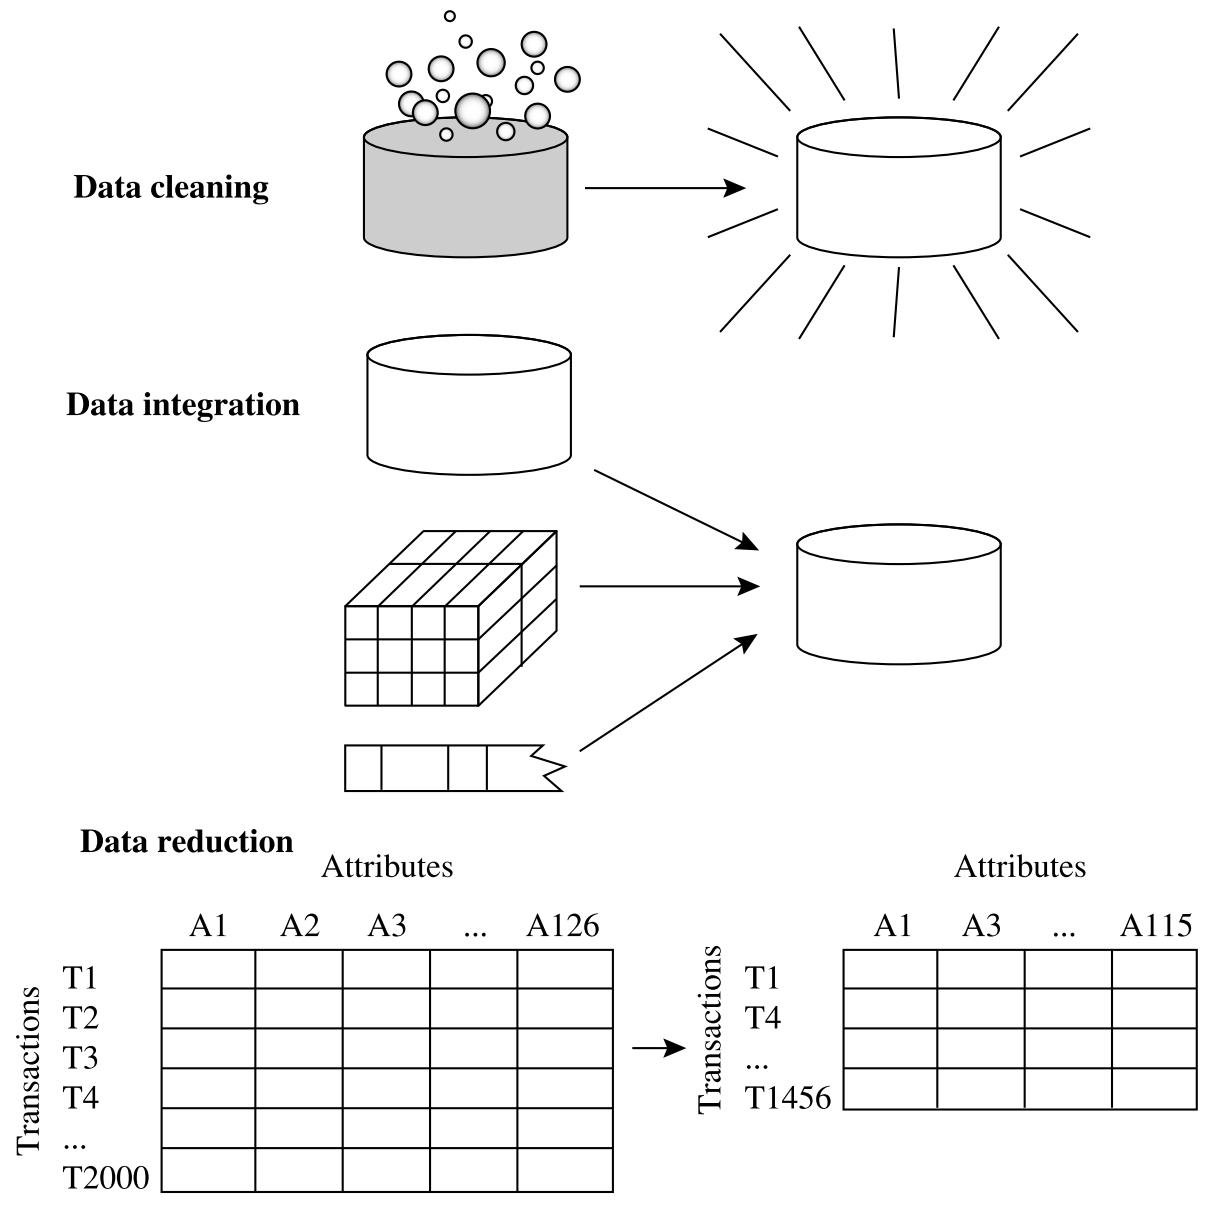
\includegraphics[scale=1.2]{se-wa-jpg/preprocessing}
\caption[Werkzeuge der Datenvorverarbeitung]{Werkzeuge der Datenvorverarbeitung\protect\footnotemark}
\label{werkzeuge}
\end{figure}
\footnotetext{Vgl. Abbildung \textit{Han}, Data Mining: Concepts and techniques, 2012, S. 87}


\subsubsection{Data Cleaning}
\label{dc}
In der realen Welt sind Daten häufig \glqq unvollständig, mit Fehlern oder Ausreißern behaftet oder sogar inkonsistent.\grqq\seFootcite{}{S. 199}{Cleve.2014} Um Fehler oder gar falsche Resultate im Data-Mining-Prozess frühzeitig zu vermeiden, ist es von großer Bedeutung, die Datenmengen zu bereinigen. Der Fokus sollte hierbei auf der Informationsneutralität liegen. Das bedeutet, es sollen möglichst keine neuen Informationen hinzugefügt werden, die das reale Abbild verzerren oder verfälschen können.\seFootcite{Vgl.}{S. 199-200}{Cleve.2014} Folgende Problemarten gilt es zu behandeln:

\paragraph{Fehlende Daten} 
Dem Datenanalyst stehen einige Möglichkeiten zur Verfügung, um auf fehlende Daten zu reagieren:\seFootcite{Vgl.}{S. 88-90}{Han.2012}\seFootcite{Vgl.}{S. 200-201}{Cleve.2014}

\begin{itemize}
\item \textit{Attribut ignorieren}
\\ Der Datensatz mit dem fehlenden Attribut wird gänzlich ignoriert oder gelöscht. Jedoch können dadurch wichtige Informationen für die Datenanalyse verloren gehen, wodurch dieses Verfahren nur bei Datensätzen mit mehreren Lücken angewandt werden sollte.

\item \textit{Manuelles Einfügen}
\\ Besitzt der Datenanalyst das nötige Wissen, kann dieser einzelne Datensätze nachträglich manuell einfügen. Dieser Vorgang entwickelt sich schnell zu einem sehr zeitaufwändigen und schwer zu realisierenden Vorgang, der aufgrund des Mangels an Ressourcen (personeller wie auch zeitlicher) nicht zu realisieren ist, sobald die Datenmenge wächst (z.B. Nachtrag von 500 Kundendaten per Hand).

\item \textit{Globale Konstante}
\\ Den fehlenden Wert durch eine globale Konstante (auch als Standardwert bezeichnet) zu ersetzen, ist sinnvoll, wenn auch ein leeres Feld als Information angesehen wird. Beispiele für Konstanten wären \textit{unbekannt} oder \textit{minus unendlich}.

\item \textit{Durchschnittswert}
\\ Handelt es sich bei dem fehlenden Attribut um einen metrischen Wert, so kann der Durchschnittswert aller Einträge als Ersatz verwendet werden. Der Durchschnittswert bietet sich als äußerst einfache Möglichkeit, wenn die Daten klassifiziert werden können und die Berechnung nur auf Datensätzen der selben Klasse angewandt wird. Die Methode der \gls{knn}\seFootcite{Vgl.}{S. 76}{Garcia.2015} steht zur Verfügung, wenn keine Klassen vorhanden sind. Hierbei wird der Durchschnitt, der dem aktuellen Datensatz ähnlichsten Werte benutzt.

\item \textit{Wahrscheinlichster oder häufigster Wert}
\\ Durch statistische Methoden kann der wahrscheinlichste Wert für das fehlende Attribut ermittelt werden, jedoch sollte diese Angleichung begründet sein. Bei nicht numerischen Werten kann als weitere Möglichkeit auch der häufigste Wert als Ersatz für das fehlende Attribut verwendet werden.
\end{itemize}

\paragraph{Verrauschte Daten und Ausreißer}
\label{outlierchapter}
Durch ungenaue Messwerte oder falsche Schätzungen entstehen die sogenannten \textit{verrauschten Daten}.\footnote{Im englischen Sprachgebrauch als \textit{noisy data} bekannt.} Um diese bereinigen zu können, stehen dem Datenanalyst einige Verfahren zur Verfügung, durch welche diese fehlerbehafteten Daten angeglichen werden können.\footnote{Auch als \textit{smoothing} bekannt.} Als \textit{Ausreißer} bezeichnet man dabei Daten, die erheblich von den anderen Daten abweichen oder außerhalb eines Wertebereiches (z.B. $0<x<100$) liegen.\seFootcite{Vgl.}{S. 89-90}{Han.2012} Beispielsweise liegen bei einer Befragung Daten von 30- bis 50-Jährigen vor, darunter auch einer von einem 90-Jährigen, könnte es sich hierbei um einen Ausreißer handeln, aber auch um einen fehlerhaften Datensatz.\seFootcite{Vgl.}{S. 196}{Cleve.2014} \glqq Ob solche Ausreißer für das Data Mining ausgeblendet oder adaptiert werden sollten oder besser doch im Originalzustand zu verwenden sind, hängt vom konkreten Kontext ab.\grqq\seFootcite{}{S. 196}{Cleve.2014}


\begin{itemize}

\item \textit{Klasseneinteilung (bining)}
\\ Durch die Gruppierung verrauschter Daten in Klassen, können diese beispielsweise durch den Mittelwert oder die naheliegenden Grenzwerte ersetzt werden. 

\item \gls{regression}
\\ Die Darstellung der Daten in Form einer mathematischen Funktion, bietet die Möglichkeit, fehlerbehaftete Daten  durch die berechneten Funktionswerte zu ersetzen. Für zwei Abhängigkeiten zwischen zwei Attributen steht hierbei neben der \textit{linearen Regression}, auch die \textit{multiple lineare Regression} für mehrere Attribute als Werkzeuge zur Verfügung (weiterführende Ausarbeitung zur Regressionsanalyse siehe \vref{ra}). 

\item \textit{Verbundbildung (clustering)}
\\ Eine der einfachsten Möglichkeiten um Ausreißer zu erkennen, bietet die Verbundbildung, auch \gls{clustering} genannt. Hierbei werden ähnliche Daten, wie in \vref{outlier} dargestellt, zu \textit{Clustern} zusammengeführt, wodurch sich die Ausreißer direkt identifizieren lassen.

\begin{figure}[H]
\centering
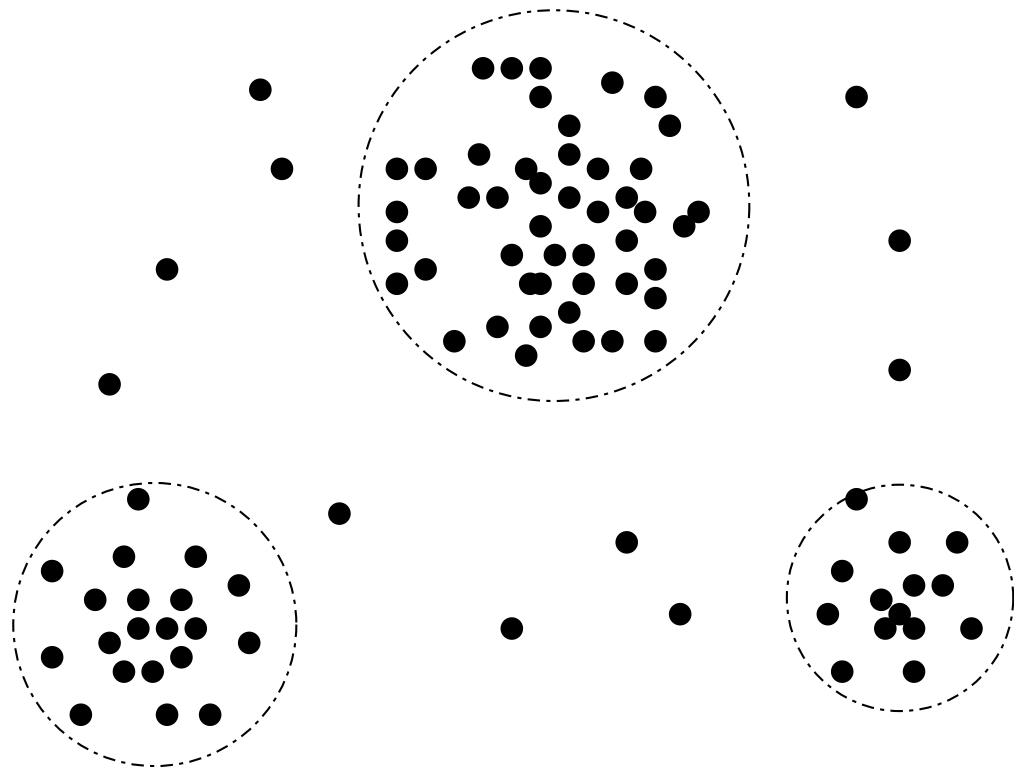
\includegraphics[scale=1.2]{se-wa-jpg/outlier}
\caption[Outlierdetection mittels Clustering]{Outlierdetection mittels Clustering\protect\footnotemark}
\label{outlier}
\end{figure}
\footnotetext{Vgl. Abbildung \textit{Han}, Data Mining: Concepts and techniques, 2012, S. 91}
\end{itemize}

\paragraph{Falsche und inkonsistente Daten}
Bei falschen bzw. inkonsistenten Daten ergeben sich prinzipiell zwei Möglichkeiten zur Korrekturbehandlung. Einerseits können der Datensatz oder bestimmte Attribute durch \textit{Löschen} entfernt werden, wobei jedoch die Gefahr einer zu großen Reduktion des Datenbestandes entsteht und relevante Informationen für das Data Mining verloren gehen könnten. Die zweite Korrekturvariante versucht den inkonsistenten Datensatz, durch die \textit{Zuhilfenahme anderer Datensätze}, sinnvoll zu ersetzen. Sollte eine Unterscheidung zwischen \textit{falsch} und \textit{richtig} nicht möglich sein, wären beim Löschen immer mindestens zwei Datensätze betroffen.\seFootcite{Vgl.}{S. 203-204}{Cleve.2014}

\subsubsection{Data Integration}
\label{di}
Bei Data-Mining-Projekten ist oftmals die Integration mehrerer Datenbestände aus unterschiedlichen Quellen erforderlich. Diese Phase sollte mit äußerster Sorgfalt durchgeführt werden, um frühzeitig redundante und inkonsistente Datensätze zu vermeiden, wodurch die Genauigkeit und Geschwindigkeit der nachfolgenden Data Mining Algorithmen nicht gefährdet wird.\seFootcite{Vgl.}{S. 93-94}{Han.2012} Folgende Punkte gilt es bei der Datenintegration zu beachten:

\begin{itemize}
\item \textbf{Identifikationsproblem von Entitäten}:
\\ Bei der Datenintegration aus multiplen Datenquellen, wie beispielsweise Datenbanken oder Dokumenten, stellt die Schema-Integration wie auch die Objektanpassungen eine schwierige Herausforderung dar. Der Datenanalyst muss sicherstellen, dass zum Beispiel das Attribut \textit{kunden\_nummer} aus der einen Datenquelle, die selbe Referenz besitzt, wie das Attribut \textit{kunden\_id} aus einer anderen und es sich folglich um das selbe Attribut handelt. Dies wird allgemein als \textit{Problem Identification Problem} bezeichnet.\seFootcite{Vgl.}{S. 199}{Cleve.2014}\seFootcite{Vgl.}{S. 94}{Han.2012} Die Metadaten der Attribute beinhalten Informationen, wie \textit{Name, Bedeutung, Datentyp, Wertebereich, uvm.} und können durch Abgleich derer zu einer Vermeidung von Fehlern bei der Integration beitragen. Weiterhin muss gesondert auf die \textit{Datenstruktur} geachtet werden, um keine referentiellen Abhängigkeiten bzw. Beziehungen zwischen den Daten zu zerstören.\seFootcite{Vgl.}{S. 94}{Han.2012} 

\item \textbf{Redundanzen bei Attributen}:
\\ Ein Attribut, welches durch ein anderes Attribut ableitbar ist -- wie zum Beispiel das Alter vom Geburtsjahr berechnet werden kann -- wird als redundant bezeichnet. Die Vielzahl von Redundanzen führt zu unnötig großen Datenmengen, die wiederum die Performanz sowie die Resultate eines Data Mining Algorithmus negativ beeinträchtigen können.\seFootcite{Vgl.}{S.41}{Garcia.2015} Folglich sollte diese Problematik durch die Anwendung von statistischen Verfahren, in Form der Korrelationsanalyse, dezidiert behandelt werden. Für numerische Werte ist dabei der Einsatz von Korrelationskoeffizienten und Kovarianzen hilfreich. Um die Implikation zweier Attribute einer nominalen Datenmenge\footnote{Rein qualitative Merkmalsausprägungen ohne natürliche Rangordnung (wie z.B. das Geschlecht).} bestimmen zu können, verwendet man in der Regel den $\chi^2$(\textit{Chi-Quadrate})-Test.\seFootcite{Vgl.}{S. 95.}{Han.2012}\seFootcite{Vgl.}{S. 41}{Garcia.2015}\seFootcite{Vgl.}{S. 64}{Cleve.2014} 

\item \textbf{Duplikatserkennung}:
\\ Duplikate verkörpern Redundanzen auf Datensatzebene und führen einerseits zu unnötig großen Datenmengen, die sich wiederum auf die Performanz der Algorithmen auswirken. Andererseits führt jedoch auch die verfälschte Gewichtung der mehrfach vorkommenden Datensätze, zu falschen Analyseergebnissen. Ein häufiger Grund stellt dabei die Verwendung von denormalisierten Datenbanktabellen dar.\seFootcite{Vgl.}{S. 98}{Han.2012}\seFootcite{Vgl.}{S. 43}{Garcia.2015}

\item \textbf{Konflikte bei Attributswerten}:
\\ Hierbei handelt es sich um die unterschiedliche Darstellung, Skalierung und Kodierung von Attributswerten. Beispielsweise kann das Attribut \textit{Gewicht} durch das metrische System oder das britische Maßsystem repräsentiert werden, woraus bei der Zusammenführung von Daten in eine einheitliche Quelle immer wieder Konflikten resultieren.\seFootcite{Vgl.}{S. 99}{Han.2012}\seFootcite{Vgl.}{S. 199}{Cleve.2014} 
\end{itemize}

\subsubsection{Data Reduction}
\label{dr}
Die bereits mehrfach angesprochene Problematik der riesigen Datenmengen bei Data-Mining-Projekten, steigert die Komplexität und vermindert die Effizienz der Algorithmen. Daher strebt die Datenreduktion -- wie die Bezeichnung erkennen lässt -- nach einer reduzierten repräsentativen Teilmenge, welche die Integrität des Originals nicht verliert. Dazu können folgende drei Techniken angewandt werden:\seFootcite{Vgl.}{S. 147 ff}{Garcia.2015}\seFootcite{Vgl.}{S. 99-100}{Han.2012}\seFootcite{Vgl.}{S. 206-208}{Cleve.2014} 

\begin{enumerate}

\item Dimensionsreduktion 

\item Datenkompression

\item Numerische Datenreduktion

\end{enumerate}

\paragraph{Dimensionsreduktion}
Hierbei bleiben irrelevante Attribute des Datensatzes unberücksichtigt und nur für die Analyse relevante Daten werden miteinbezogen. Allgemein empfehlen sich dafür zwei Verfahren: Bei der schrittweisen \textit{Vorwärtsauswahl} werden wesentliche Attribute einer sukzessiv wachsenden Zielmenge zugeordnet. Im Gegensatz dazu werden bei der \textit{Rückwärtseliminierung} die uninteressanten Daten schrittweise aus der Zielmenge eliminiert.\seFootcite{Vgl.}{S. 206}{Cleve.2014} 

\paragraph{Datenkompression}
\label{datenkompression}
Bei dieser Technik wird durch Transformation oder Codierung versucht, eine Reduktion der Datenmenge zu erreichen. Fasst man beispielsweise die einzelnen Attribute \textit{Tag, Monat und Jahr} zu einem neuen Attribut \textit{Datum} zusammen, können Datensätze komprimiert werden.\seFootcite{Vgl.}{S. 207}{Cleve.2014}
 
\paragraph{Numerische Datenreduktion}
Statt die gesamte Datenmenge für die Analyse heranzuziehen, wird innerhalb der numerischen Datenreduktion eine repräsentative Teilmenge -- in Form einer Stichprobe -- für das \gls{dm} genutzt. Im Vordergrund steht hierbei die passende Auswahl unterschiedlicher Stichprobeverfahren, wie der \textit{zufälligen Stichprobe} oder der \textit{repräsentativen Stichprobe}, woraus jedoch kein verzerrtes Abbild der Daten resultieren darf.\seFootcite{Vgl.}{S. 25-27}{Fahrmeir.2007}\seFootcite{Vgl.}{S. 207}{Cleve.2014}
\subsection{Datentransformation}
\label{dt}
Nachdem die (Roh-)Daten selektiert, bereinigt und auf eine relevante Zielmenge reduziert wurden, müssen diese noch in eine adaptierte Form für die Algorithmen des Data Minings transformiert werden.\seFootcite{Vgl.}{S. 112}{Han.2012} Oftmals müssen sogar neue Attribute aus einem Datensatz kreiert werden, da dieser nicht in geeigneter Struktur für das Data-Mining-Verfahren vorliegt.\seFootcite{Vgl.}{S. 48}{Garcia.2015} Dazu gibt es eine Reihe an unterschiedlichen Transformationsmöglichkeiten, wobei in dieser Arbeit ein Auszug der relevanten Methoden vorgestellt werden soll:

\paragraph{Codierung}
Liegen beispielsweise Attribute mit einer ordinalen Ausprägung vor (wie \textit{sehr groß, groß, mittel und klein}), müssen diese bei einer Verwendung des \gls{knn}-Algorithmus in numerische Werte transformiert werden (Werte zwischen 0 und 1). Hierbei würde sich folgende Codierung für das Attribut \textit{Körpergröße} anbieten:\seFootcite{Vgl.}{S. 210}{Cleve.2014}

\begin{itemize}
\item \textit{sehr groß} $\rightarrow$ 1
\item \textit{groß} $\rightarrow$ 0,66
\item \textit{mittel} $\rightarrow$ 0,33
\item \textit{klein} $\rightarrow$ 0
\end{itemize}

Die Ordnungsrelation, hier \textit{sehr groß > groß > ...}, darf dabei jedoch nicht verloren gehen. In Abhängigkeit zu dem jeweiligen Verfahren, müssen Daten, so wie dies bei Maßeinheiten immer wieder der Fall ist, oftmals kodiert werden.\seFootcite{Vgl.}{S. 211}{Cleve.2014}

\paragraph{Normalisierung und Skalierung}
Unterschiedliche Maßeinheiten -- wie \textit{Körpergröße} und \textit{Körpergewicht} -- können die Datenanalyse negativ beeinflussen und müssen daher in eine einheitliche Skalierung transformiert werden, um eine gleiche Gewichtung aller Attribute zu erreichen. Man bedient sich hierbei in der Regel an der \textit{Min-Max-Normalisierung} (siehe \vref{minmax}) oder der \textit{Z-Transformation}, um numerische Werte auf ein [0,1] Intervall zu normieren.\seFootcite{Vgl.}{S. 114}{Han.2012}\seFootcite{Vgl.}{S. 212}{Cleve.2014}

\begin{figure}[H]
\begin{equation}
x_{neu} = \frac{x - min(x_i)}{max(x_i) - min(x_i)}
\end{equation}
\caption{Min-Max-Normalisierung}
\label{minmax}
\end{figure}

\paragraph{Datenaggregation}
Nicht nur aus Sicht der Datenkompression (vgl. \vref{datenkompression}) ist die Datenaggregation erforderlich. Vielmehr \glqq kann die Aggregation aus inhaltlichen Gründen sinnvoll sein.\grqq\seFootcite{}{S. 214}{Cleve.2014} Wenn Daten auf einer zu detaillierten Ebene vorliegen -- wie beispielsweise Einwohnerzahlen von Stadtteilen -- müssen diese für einen Städtevergleich erst summiert werden, um bundesweite Aussagen treffen zu können. Je nach Kontext können verschiedene Aggregationsmethoden (wie z.B. Summenbildung, Durchschnitt, usw.) für die Transformation zu einem einzigen Wert angewendet werden.\seFootcite{Vgl.}{S. 112}{Han.2012}

\paragraph{Datenglättung}
Die bereits in \vref{outlierchapter} vorgestellten Techniken zur Bereinigung von verrauschten Daten und Ausreißern, finden auch bei der Transformation ihre Verwendung. Die Datenglättung strebt nach einer reduzierten Datenmenge, in welcher jeder numerische Wert durch einen idealisierten Wert, wie beispielsweise der \textit{\gls{regression}}, ersetzt wird.\seFootcite{Vgl.}{S. 214-215}{Cleve.2014}
\subsection{Data-Mining-Methoden}
\label{dmmethoden}

Nachdem die Daten in geeigneter Form vorliegen, kommt das eigentliche Herzstück des \gls{kdd}-Prozesses -- das \textit{Data Mining} -- zum Tragen. In diesem Schritt wird zu nächst überprüft, welche grundlegende Data-Mining-Aufgabe es zu lösen gilt, um anschließend ein passendes Analyseverfahren zur Identifizierung von Mustern und Zusammenhängen auswählen zu können.\seFootcite{Vgl.}{S. 10}{Cleve.2014} Die interdisziplinäre Wissenschaft des Data Minings umfasst bewährte Techniken aus mehreren Forschungsgebieten, welche auf verschiedenste Problemfälle der Realität, wie Zeitreihenanalysen, Funktionsmodellierungen, Klassifikation uvm., angewendet werden können. Grundsätzlich basieren fast alle Analyseverfahren auf der Mathematik, insbesondere der Statistik.\seFootcite{Vgl.}{S. 12}{Cleve.2014} Im Allgemeinen unterteilt man die Data-Mining-Methoden in zwei Kategorien: \textit{Prognose} und \textit{Beschreibung}. Hierzu gibt \vref{dmmethods} einen Überblick über die Einteilung der etablierten Methoden, welche im Folgenden kurz aufgeführt werden.

\paragraph{Prognose:} In dem Bereich der Prognose unterscheidet man zwischen zwei Gruppen: \textit{statistische Methoden} und \textit{symbolische Methoden}. Letztere versuchen das Wissen durch Symbolik und Verknüpfung, auf einer leichter interpretierbaren Ebene für Menschen, zu vermitteln. Im Gegensatz dazu, repräsentieren statistische Methoden das Wissen mit Hilfe der Erstellung von mathematischen Modellen.\seFootcite{Vgl.}{S. 3}{Garcia.2015} Die am häufigsten angewendeten statistischen Methoden sind folgende:\seFootcite{Vgl.}{S. 3-5}{Garcia.2015}\seFootcite{Vgl.}{S. 23-24}{Han.2012}

\begin{itemize}
\item \textit{Regressionsanalyse}
\\ Die älteste \gls{dm}-Methode dient zur Funktionsmodellierung von einer abhängigen oder mehreren unabhängigen Variablen. Die Form der Funktion wird dabei durch das ausgewählte Verfahren, beispielsweise \textit{lineare oder quadratische Regression}, bestimmt und kann anhand bestimmter Parameter validiert werden, wie \glqq gut\grqq~diese zu den eingebrachten Daten passt.\seFootcite{Vgl.}{S. 3}{Garcia.2015}

\item \textit{(Künstliche)} \gls{nn}
\\ In diesem Teilbereich der künstlichen Intelligenz wird versucht, einen Wissensspeicher zu kreieren, der ähnlich unserem leistungsfähigen Gehirn funktioniert. Hierbei werden die biologischen Elemente und Vorgehensweise des Gehirns, in Form von \textit{Neuronen}, in die Welt des Computers übertragen. Durch gerichtete und gewichtete Verbindungen sind diese Neuronen untereinander verknüpft und bilden so ein gemeinsames Netz für die Informationsverarbeitung.\seFootcite{Vgl.}{S. 47}{Cleve.2014}

\item \gls{svm}
\\ Die auf \gls{ml} basierende Methode versucht Objekte zu klassifizieren. Dabei werden alle Objekte als Vektoren in einem Raum dargestellt und durch sogenannte \textit{Hyperebenen} (fungieren als Trennflächen) geteilt, um eine möglichst zuverlässige Zuordnung der Daten in vordefinierte Klassen zu erreichen.\seFootcite{Vgl.}{S. 313}{Aggarwal.2015}
\end{itemize}

Im Bereich der symbolischen Methoden hat sich die Technik des \textit{Entscheidungsbaumes} etabliert. Sie dient ebenfalls der Klassifizierung von Objekten, indem innerhalb jedes Iterationsschrittes das am \textit{besten} zu klassifizierende Attribut gefunden wird, um die Daten daran aufzusplitten. Durch dieses Verfahren entsteht ein Entscheidungsbaum, von dem Regeln, wie \textit{If-Else-Zweige}, abgeleitet werden können.\seFootcite{Vgl.}{S. 5}{Garcia.2015}

\paragraph{Beschreibung:}

\begin{itemize}
\item \textit{Clustering}
\\ Im Gegensatz zur Klassifizierung sind bei der Methode des Clustering zuvor keine Klassen bzw. Gruppen definiert. Dieses weitverbreitete Werkzeug im Bereich des Data Minings versucht Daten in sogenannte \textit{Cluster} zu unterteilen, wobei die Elemente dieser Gruppen sich möglichst ähnlich (\textit{homogen}), jedoch auch gleichzeitig von den anderen Clustern deutlich zu unterscheiden sein sollten (\textit{heterogen}).\seFootcite{Vgl.}{S. 3}{Anderberg.2014}
\enlargethispage{\baselineskip} 
\item \textit{Assoziationsanalyse}
\\ Diese Methode versucht Wissen durch assoziative Beziehungen zwischen den Daten herzuleiten. Das einfachste Beispiel hierfür wäre im Einzelhandelsbereich: \glqq Wenn ein Kunde Produkt A kauft, würde dieser auch Produkt B kaufen.\grqq~Durch diese extrahierten Muster, können wiederum Regeln abgeleitet werden.
\end{itemize}


\paragraph{Visualisierung als Werkzeug:}
Nicht zuletzt ist die Visualisierung unerlässlich für den Erfolg eines Data-Mining-Projektes. Die Resultate werden oftmals zur Entscheidungsfindung herangezogen, wobei die Entscheidungsträger nicht immer direkt am Prozess beteiligt sind. Die Ergebnisse müssen folglich in einer anschaulichen und nachvollziehbaren Form dargestellt werden, um Vertrauen und Akzeptanz in die Resultate zugewinnen.\seFootcite{Vgl.}{S. 14}{Cleve.2014} Weiterhin kann die Visualisierung auch schon in der Datenvorverarbeitung genutzt werden oder als eigenständige Methode innerhalb des Data Minings, da sich häufig erst Zusammenhänge zwischen den Attributen durch die Darstellung der Daten erkennen lassen.\seFootcite{Vgl.}{S. 14}{Cleve.2014}

\paragraph{Auswahl der Methode:}
Für die Modellierung einer Funktion zur Berechnung der Wahrscheinlichkeit eines Torerfolges im Fußball (auch bekannt unter dem Begriff \textit{Expected Goals}), kann die passende Data-Mining-Methode aus der \vref{dmmethods} ausgewählt werden. Der zu erwartende Torerfolg soll folglich prognostiziert und durch ein mathematisches Modell repräsentiert werden. Unter den statistischen Methoden eignet sich für die Modellierung einer Funktion am besten die Regressionsanalyse, da ein Torerfolg von mehreren Faktoren abhängig ist. Dementsprechend wird dieses Verfahren als Data-Mining-Methode für die Beantwortung der vorliegenden Problemstellung ausgewählt und dessen Bestandteile zunächst in \vref{fm} betrachtet, um diese Technik in der späteren Umsetzung anwenden zu können.	

\begin{sidewaysfigure}
\centering
\includegraphics[scale=0.34]{se-wa-jpg/dmmethods}
\caption[Übersicht: Data-Mining-Methoden]{Übersicht: Data-Mining-Methoden\protect\footnotemark}
\label{dmmethods}	
\footnotetext{Abbildung in Anlehnung an \textit{García} et al., Data preprocessing in data mining, 2015, S. 4.}
\end{sidewaysfigure}
\subsection{Interpretation}
Am Ende des \gls{kdd}-Prozesses steht die Interpretation sowie die Evolution der entdeckten Muster und Beziehungen aus dem Data Mining. Oftmals können Unternehmen keinen Nutzen aus den Analyseverfahren erzielen, da diese häufig irrelevante, triviale, bedeutungslose oder sogar bereits bekannte Daten generieren. Die gewonnenen Muster sollten den folgenden vier Kriterien genügen, um neues Wissen zu repräsentieren:\seFootcite{Vgl.}{S. 11-12}{Cleve.2014}

\begin{enumerate}
\item \textbf{Validität:} Hierbei wird die Gültigkeit des Muster für das gefundene Modell, als auch in Bezug auf neue Daten, in einem objektives Maßstab beschrieben.
\item \textbf{Neuartigkeit:} Das Kriterium beantwortet die Frage, inwiefern das neu erworbene Wissen zu den bisherigen Forschungen steht. Einerseits es kann den Wissensstand ergänzen oder im Widerspruch dazu stehen.
\item \textbf{Nützlichkeit:} Beschreibt das Nutzen, welches für den Anwender durch die Resultate erzielt wurde.
\item \textbf{Verständlichkeit:} Die Ergebnisse des Modells sollten von einem anderen Anwender verstanden werden.
\end{enumerate}

Anhand dieser Anforderungen sollen die späteren Ergebnisse der modellierten Funktionen gemessen werden. Um dabei eine aussagekräftige Interpretation der Ergebnisse treffen zu können, erfordert es ein hohes Maß an Verständnis der vorliegenden Problemstellung. Zu bietet sich ein Team von Experten an, welche die Resultate validieren, sodass eine korrekte Bewertung erzielt wird. Für die Interpretationsphase eignet sich die Verwendung von Werkzeugen, wie der Visualisierung, um schnellen Aufschluss über die gewonnenen Muster und Zusammenhänge zu erlangen. Innerhalb des iterativen \gls{kdd}-Prozesses (siehe \vref{kddpic}) ist ein Rücksprung die vorherigen Phasen typisch.\seFootcite{Vgl.}{S. 11}{Cleve.2014} Meist müssen Daten nochmal nachbereitet, eine andere Data-Mining-Methode ausgewählt oder sogar Daten neu selektiert werden, wenn das gewünschte Ergebnis sich mit der verwendeten Datenbasis nicht erreichen lässt.\seFootcite{Vgl.}{S. 11}{Cleve.2014}
\chapter{Zusammenfassung}

\section{Fazit}
Im Rahmen der vorliegenden Arbeit konnte gezeigt werden, wie Methoden des Data Minings innerhalb eines strukturierten Prozesses im Bereich der Datenanalyse im Fußball eingesetzt werden können, um neues Wissen zu schaffen. Durch den systematischen Aufbau des Knowledge Discovery in Data Prozesses und den darin beinhaltenden Methoden zur Verbesserung der Datenqualität konnte aus der rohen Datenmenge, gemäß den Anforderungen, eine valide und fundierte Funktion modelliert werden, die die Wahrscheinlichkeit für einen Torerfolg eines Schusses aus jeder möglichen Position auf dem Spielfeld berechnet. 

Im Zuge der vorbereitenden Schritte der Datenselektion, -vorverarbeitung und -transformation wurde in der Umsetzung deutlich, wie essentiell diese Phasen für die Qualität der Resultate des Data Minings sind. So konnten die Eigentore, die zuvor kein Bestandteil der Anforderungen waren, nachträglich ausgeschlossen und Ausreißer in der Datenmenge identifiziert oder das Problem der weißen Linien aufgedeckt werden. Aus der vergleichenden Analyse der modellierten Funktionen resultiert, dass die Verwendung des \textit{nichtparametrischen} Regressionsmodells in Form sogenannter \textit{Splines} in Kombination mit der Betrachtung der Koordinaten des Schusses besonders geeignet ist und zu einer genauen Anpassung des Modells an die Daten führt. In Bezug auf die Betrachtung des Winkels und der Distanz des Schussversuches zum Tor erwies sich weder das \textit{multiple} noch das \textit{nichtparametrische} Regressionsmodell als valide. Die Ergebnisse der Evaluation beweisen, dass mit lediglich zwei Parametern, den Koordinaten des Schusses, eine gute Balance zwischen einem Under- bzw. Overfitting des Modells gefunden werden konnte. Das Software-Tool MATLAB bestätigte des Weiteren die weltweit erstklassige Reputation mit den bereitgestellten Bibliotheken zur Regressionsanalyse, sowie deren intuitiven und benutzerfreundlichen Bedienung. \enlargethispage{2\baselineskip} 

Die erstmalige Modellierung der \textit{Expected Goals} durch eine Funktion bietet die Basis für ein datenbasiertes und objektiv bewertetes Scouting, sowie weitere nützliche Anwendungsfälle, die im nachfolgenden Ausblick in \vref{ausblick} behandelt werden.



\section{Ausblick}
\label{ausblick}

Die vorliegende erarbeitete Funktion wurde anhand der Daten aus der deutschen Bundesliga modelliert und ist somit auch zunächst lediglich für diese Fußballliga gültig. Das Modell könnte dahingehend erweitert werden, dass für jede europäische Topliga ein eigenes Modell erstellt wird, um Muster zwischen diesen Ländern erkennen zu können. In Bezug auf einen Spieler ergeben sich weitere alternative Anwendungsmöglichkeiten. Werden beispielsweise alle Schüsse eines Spielers in die Funktion eingesetzt, ergibt sich daraus der erwartete Wert an Toren. Dieser Wert wird mit den tatsächlich erzielten Toren verglichen, um statistisch belegte Aussagen über die Erfolgsquote des Spielers treffen zu können, welche für oder gegen dessen Qualität sprechen. Des Weiteren bietet dieses Modell die Grundlage auch Defensivaktionen, wie zum Beispiel gewonnene Zweikämpfe, in einen neuen Maßstab zu setzen, da durch den Ballbesitzwechsel die gegnerische Mannschaft aus der vorherigen Position kein Tor mehr schießen kann. Beispielsweise konnte ein Abwehrspieler die siebzig-prozentige Wahrscheinlichkeit auf einen Torerfolg aus fünf Metern Distanz mit einem gewonnenen Zweikampf verhindern, wodurch seine Kennzahl steigt. Im Gegensatz dazu würde ein verlorener Zweikampf in dieser Situation seinen KPI negativ belasten.

In Bezug auf die vorgestellte Anwendung innerhalb des Scoutingbereiches im Fußball, ergibt sich die Frage, inwieweit ein solches Modell einen Scout ersetzen beziehungsweise dessen Aufgaben automatisiert ausführen kann. Diese Frage lässt sich teilweise mit ja beantworten. Möchte ein Verein einen neuen Stürmer verpflichten und verfügt dabei über ein limitiertes Budget, so kann mit Hilfe dieses Modelles eine automatisierte Vorselektion passender Spieler durchgeführt werden, wodurch die Anzahl an der dafür benötigten Scouts reduziert werden kann. Eine subjektive Einschätzung des Spielers muss letztlich immer erfolgen, sodass eine vollständige Ersetzung der Funktion des Scouts auch in Zukunft ausgeschlossen werden kann. Zu viele nicht objektiv messbare Indikatoren, wie taktisches Spielverständnis oder Teamfähigkeit, spielen eine entscheidende Rolle bei der Verpflichtung eines neuen Spielers. Dieses Modell soll nicht das fußballerische Expertenwissen des Scouts ersetzen, sondern subjektive Wahrnehmungen, die jedoch durch solch eine Funktion objektiv messbar sind, validieren und alltäglich anstehende Aufgaben erleichtern. Zusätzlich können Algorithmen entworfen werden, die automatisiert auf dem Transfermarkt nach sogenannten \glqq Schnäppchen\grqq~oder verborgenen Talenten suchen, die für einen relativ günstigen Preis dadurch verpflichtet werden können. 

Nicht zuletzt dient diese Modellierung auch als Erfahrungsgrundlage für weitere zukünftige Modelle, die aus der großen rohen Datenmenge, die durch neueste Technologien im Fußball erhoben werden, neues Wissen schaffen.


% Anhang der Arbeit
% 
%
\seAppendix{}

\newcommand{\waInputStyles}{\texttt{se-wa-input-styles-v097.tex}}

\chapter{Annahmen}
\chapter{MatLab Code}

%
%  Erzeugung eines Glossars
%
% Achtung: Das Glossar wird nur ausgegeben, wenn mindestens ein Eintrag in der Arbeit 
%                definiert wurde
%
%
\newpage
\sePrintGlossary{}


%
% Literaturverzeichnisses
%
%\newpage
\sePrintBibliography{}

%%  Erzeugung von Eintr\"agen im Literaturverzeichnis
%
%  Achtung: in einer Seminar-/Projekt/Bachelorarbeit darf da \nocite-Kommando nicht verwendet werden,
%                 da es einen Eintrag im Literaturverzeichnis erzeugt, ohne dass eine 
%                 entsprechende Literaturreferenz im Text der Arbeit angegeben wird
%
%
%
\nocite{DHBW:SG}
\nocite{KM:KS}
\nocite{Dud06}
\nocite{Dud09}
\nocite{Bri:WA}
\nocite{RP:WA}
\nocite{Sch:WAS}
\nocite{BSS:WA}
\nocite{Kor:WA}
\nocite{MK:GWA}
\nocite{ADG:WA}
\nocite{The:WA}
\nocite{BA:WA}
\nocite{Dij:CRT}
\nocite{BC:Cur}
\nocite{Par:ECP}
\nocite{Bro:SBE}
\nocite{GI:ADI}
\nocite{GI:AZI}
\nocite{Den:CD}
\nocite{LMS:Icb}
\nocite{Fre:SIF}




%
% Festlegung des grundlegenden Formatierungsstils des Literaturverzeichnis
%
\bibliographystyle{jurabib}

% Eigentliche Ausgabe der in der Arbeit verwendeten Quellen
%
%
% Angabe der bib-Dateien, in denen die Quellen beschrieben sind;
% die Angabe geht davon aus, dass eine wa.bib-Datei in demselben 
% Verzeichnis liegt, wie se-ba-vorlage.tex
%

% 2016-04-01
%
% Umbenennung von Quellen- in Literaturverzeichnis (nicht empfohlen, da sich 
% die 
% 
\renewcommand*{\bibname}{Literaturverzeichnis}
\seBibliography{wa}


%
% Erzeugung der ehrenw\"ortlichen Erkl\"arung
%
% Der optionale Parameter kann verwendet werden, um f\"ur das Thema der Arbeit eine 
% andere Formatierung vorzunehmen; das sollte in der Regel nicht erforderlich sein;
% ausserdem besteht die Gefahr inkonsistenter Titel auf dem Titelblatt und in der 
% ehrenw\"ortlichen Erkl\"arung
%
\seEhrenwoertlicheErklaerung{} % dieses Kommando sollte standardm\"assig verwendet werden
%\seEhrenwoertlicheErklaerung[\LaTeX-Vorlage zur Anfertigung \seThemaWaArbeit{} (Version \version{})]


\end{document}











